% Advay: data, least-squares baseline, held-out evaluation and limitations.
% Drop-in file:  % Advay: data, least-squares baseline, held-out evaluation and limitations.
% Drop-in file:  % Advay: data, least-squares baseline, held-out evaluation and limitations.
% Drop-in file:  % Advay: data, least-squares baseline, held-out evaluation and limitations.
% Drop-in file:  \input{advay_data_validation_section}   (standalone build: advay_main.tex)
% Figures: graphs/advay_*.{eps,pdf}; table: tables/advay_heldout_metrics.tex.
\section{Data, Least-Squares Baseline and Validation}\label{sec:advay}

This section states what the historical observations are, how they were prepared, how the
model was fitted to them by nonlinear least squares, and how well the fitted model forecasts
years it never saw. Every analysis choice that could be influenced by the held-out years was
written down and committed to the project repository before those years were opened.

\subsection{Data source and meaning}\label{sec:advay-data}

We use annual counts of snowshoe hare and Canadian lynx pelts traded by the Hudson's Bay
Company, 1900--1920, in thousands of pelts, as distributed with the Stan case study
\cite{carpenter2018}. Carpenter traces the numbers through Howard's lecture notes
\cite{howard2009} to a biology textbook; the original source is the Company's fur returns,
discussed by Hewitt \cite{hewitt1921}. The values are used unchanged
(\texttt{data/historical/pelts\_1900\_1920.csv}); the file's provenance, checksums and every
transformation (removing comment lines, reordering columns) are recorded alongside it.

These are \emph{trade counts}, not censuses. Trapping effort, fur prices, the number of
reporting posts and animal behaviour all affect them; Hewitt notes that hungry lynx are
easier to trap when hares are scarce. A second widely used compilation, the tsibbledata
\texttt{pelt} series \cite{tsibbledata_pelt}, differs noticeably over the same years
(Figure~\ref{fig:advay-sources}): the correlation between the two is 0.81 for lynx but only
0.32 for hare, and individual hare values differ by more than our forecast errors. We use
the Stan series because the project protocol names it, and treat the disagreement as a source
of uncertainty that no model in this report can remove.

\begin{figure}[ht]
\centering
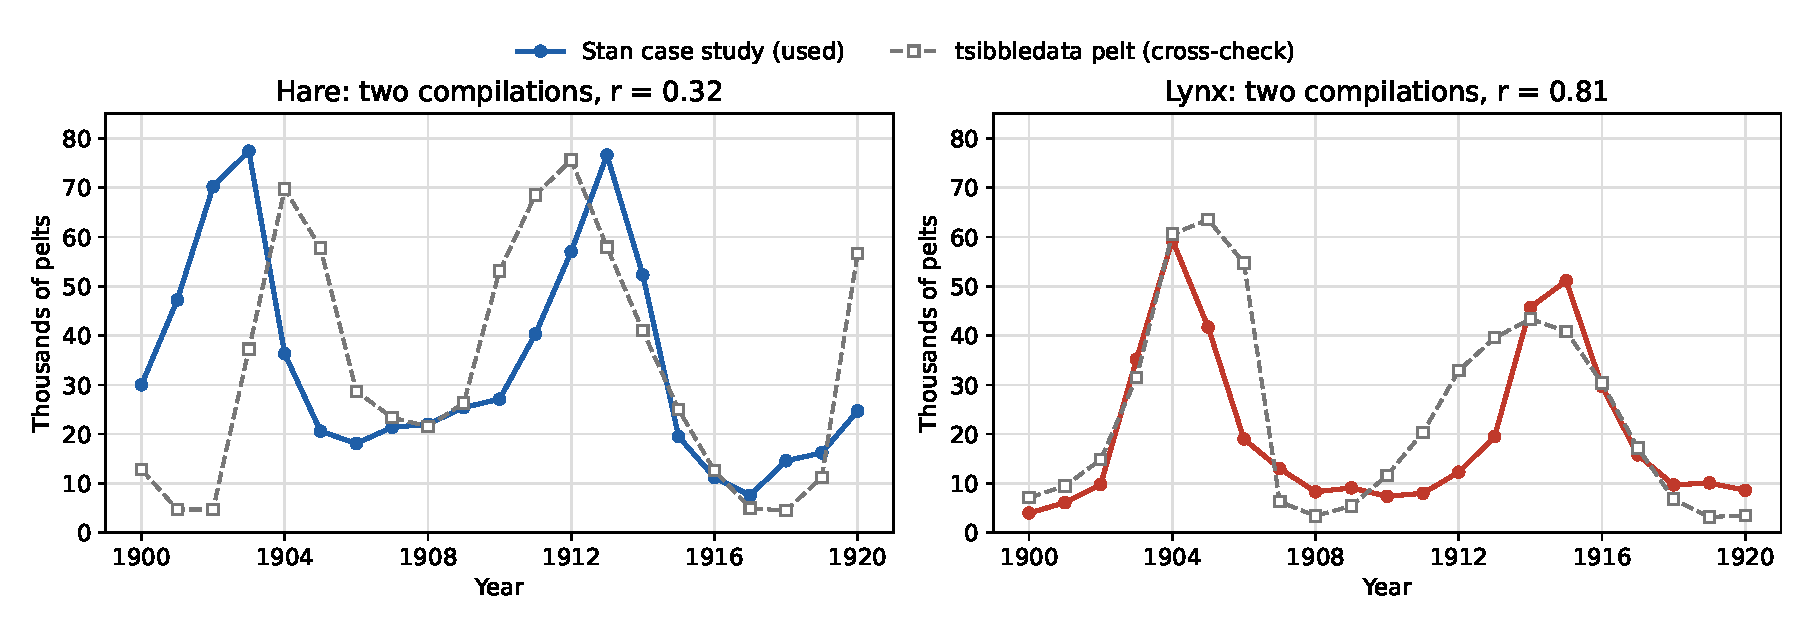
\includegraphics[width=\textwidth]{advay_source_comparison}
\caption{The Stan case-study series used here (solid) and the tsibbledata \texttt{pelt}
compilation (dashed) for 1900--1920. Both show two cycles, but yearly values differ,
especially for hare.}\label{fig:advay-sources}
\end{figure}

\paragraph{Observation model.} Following the agreed convention (assumption O1), pelt counts
are taken to be proportional to animal numbers with unknown constant factors, and the model
states are defined directly in pelt units:
\[
Y_{H,i}=H(t_i)+\varepsilon_{H,i},\qquad Y_{P,i}=P(t_i)+\varepsilon_{P,i},\qquad t_i=\mathrm{Year}_i-1900,
\]
with each annual total treated as a sample of the state at $t_i$. No observation scale factor
is fitted. Under O1, $r$, $m$ and the dimensionless groups of the model section are unchanged
by the unknown factors; $K$, $b$, $a$ and $e$ are \emph{effective} coefficients in pelt
units and are not interpreted as absolute biological quantities.

\subsection{Preparation and exploratory checks}\label{sec:advay-checks}

The 21 rows are consecutive, with no missing values, no zeros and no duplicates. The data
were split once into a training file (1900--1915, 16 rows) and a test file (1916--1920,
5 rows), with checksums recorded; all fitting code reads only the training file. Every
statistic below uses the training years only.

\begin{itemize}
\item \textbf{Cycles and lag.} Hare peaks in 1903 and 1913 (a ten-year spacing); lynx peaks
in 1904 and at the 1915 boundary. The correlation of $H(t)$ with $P(t+k)$ is largest at
$k=2$ years ($r=0.94$; $0.76$ at $k=1$). In the hare--lynx plane the data trace
counter-clockwise loops, as predator--prey models predict (Figure~\ref{fig:advay-raw}).
\item \textbf{Outliers.} None: robust $z$-scores of year-to-year log growth stay below 3
(largest 2.94, the 1903--1904 hare crash).
\item \textbf{Scale.} Training ranges are 18.1--77.4 (hare) and 4.0--59.4 (lynx). Hare counts
are about twice lynx counts, so residuals are divided by each species' training maximum
$(s_H,s_P)=(77.4,59.4)$ to weight the species equally. No log transform is used in the main
analysis; a log-residual fit is a declared sensitivity check.
\item \textbf{Split position.} Training ends exactly at the 1915 lynx peak, so the test years
are the following crash and the start of recovery: a turning point the fit never sees in
that cycle.
\end{itemize}

\begin{figure}[ht]
\centering
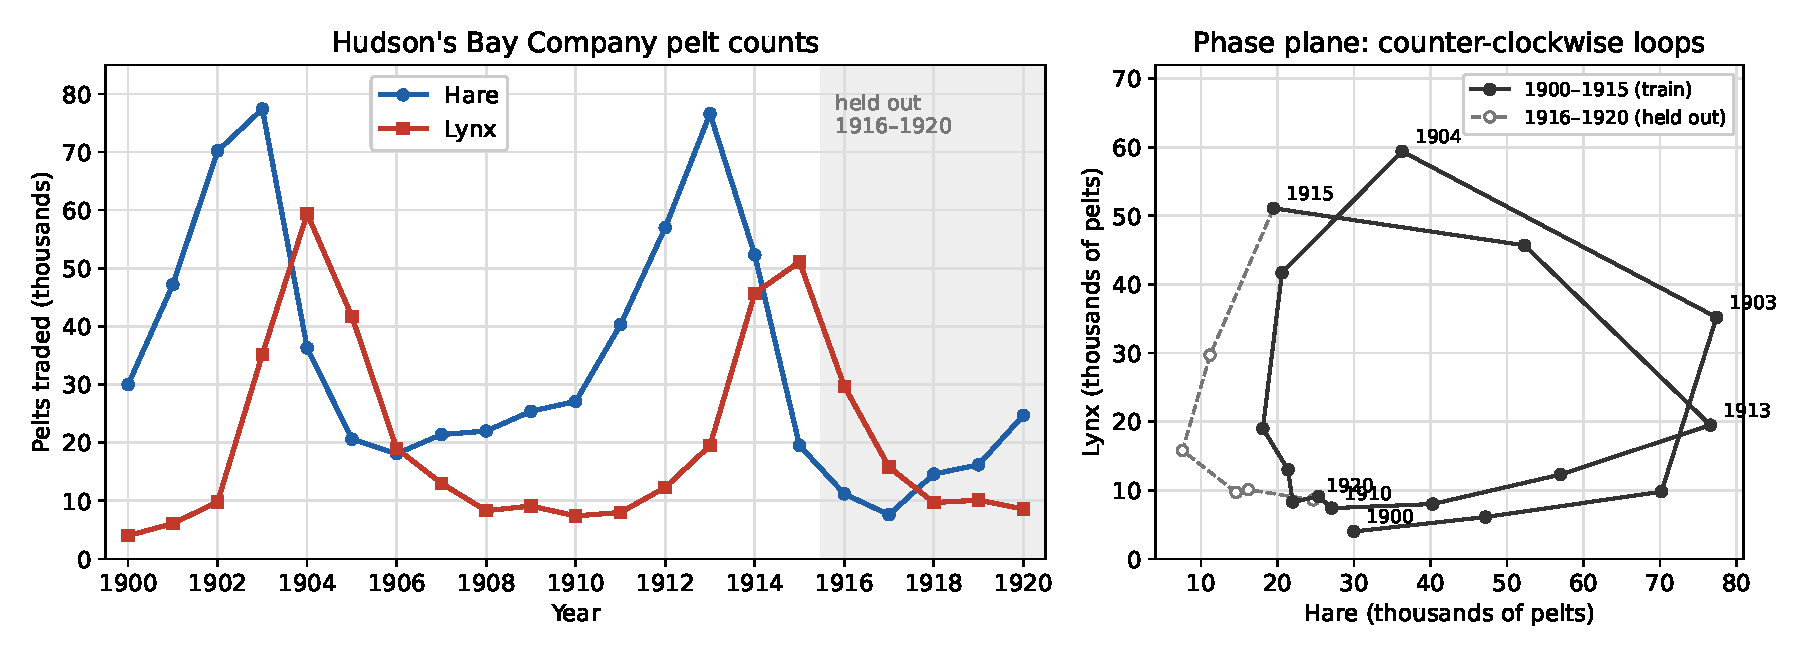
\includegraphics[width=\textwidth]{advay_raw_series}
\caption{Left: annual pelt counts, 1900--1920; the shaded band is held out. Right: the same
data in the hare--lynx plane (training solid, held-out dashed).}\label{fig:advay-raw}
\end{figure}

\subsection{Least-squares baseline}\label{sec:advay-ls}

\paragraph{Problem.} With $\theta=(r,K,a,b,e,m)$ and the shared RK45 solver (relative
tolerance $10^{-8}$, absolute $10^{-10}$, maximum step $0.1$ years), let $\hat H(t;\theta)$,
$\hat P(t;\theta)$ solve the model from the observed 1900 state $(30.0,4.0)$. The main
estimate minimises
\[
C(\theta)=\tfrac12\sum_{i=1900}^{1915}\Big[\big(\tfrac{\hat H(t_i;\theta)-Y_{H,i}}{s_H}\big)^2+
\big(\tfrac{\hat P(t_i;\theta)-Y_{P,i}}{s_P}\big)^2\Big]
\]
over the shared box bounds $r,m\in[0.05,3]$, $K\in[20,500]$, $a\in[0.05,10]$,
$b\in[0.5,300]$, $e\in[0.02,5]$. Two declared sensitivity variants change one assumption
each: \emph{log errors} replaces the scaled residuals by $\log\hat Y-\log Y$, and
\emph{fitted 1900 state} adds $(H_0,P_0)$ as unknowns within $[0.5,1.5]$ times the observed
values.

\paragraph{Method.} The bounded trust-region reflective algorithm (SciPy
\texttt{least\_squares}) is run in log-parameter space $x=\log\theta$, because the bounds
span up to a 600-fold range. Finite-difference steps of $10^{-4}$ in $x$ stay well above the
solver tolerance. The objective is multimodal, so each variant uses 80 starts: the shared
initial guess, 39 Latin-hypercube points uniform in $\log\theta$ and 39 uniform in $\theta$.
The fit with the lowest training cost is selected.

\paragraph{Protocol record.} The settings were committed before the first run. That run
(40 log-space starts) missed the best \emph{fitted 1900 state} fit, which an independent
benchmark had found at training cost $0.063$ against our $0.70$; evaluating our objective at
the benchmark's parameters gave $0.063$, so the code agreed and the start design was at
fault (the optimum sits near the upper bounds, which log-uniform starts rarely visit). The
uniform-scale starts were added as a declared amendment, judged on training cost alone and
before any test score of the baseline was computed. Both runs are kept.

\begin{table}[ht]
\centering
\begin{tabular}{lrrrrrrrl}
\toprule
Variant & $C$ & $r$ & $K$ & $a$ & $b$ & $e$ & $m$ & $\sigma=K/K_H$\\
\midrule
Main & 0.0845 & 0.647 & 382 & 10.0$^*$ & 300$^*$ & 0.967 & 0.857 & 1.07 (cycle)\\
Log errors & 0.903 & 0.520 & 197 & 7.17 & 300$^*$ & 1.80 & 1.15 & 0.55 (damped)\\
Fitted 1900 state & 0.0634 & 0.520 & 362 & 8.15 & 300$^*$ & 1.32 & 1.05 & 0.99 (damped)\\
\bottomrule
\end{tabular}
\caption{Least-squares estimates. $^*$ at the upper bound. Units: $r,m$ per year; $K,b$
thousands of hare pelts; $a,e$ effective pelt-unit coefficients. The fitted 1900 state in the
last variant is $(37.1,3.64)$.}\label{tab:advay-ls}
\end{table}

\paragraph{Results.} Table~\ref{tab:advay-ls} and Figure~\ref{fig:advay-fit} give the selected
fits. Three findings matter for interpretation.
\begin{enumerate}
\item \emph{The optimum is computationally well defined.} In every variant all starts within
1\% of the best cost (18, 42 and 16 of 80) found the same parameters to four significant
figures, and a separately written least-squares code by another team member reaches the same
optimum (training costs within $2\times10^{-7}$, forecasts within 0.002 thousand pelts).
\item \emph{The saturation of predation is not identified.} $b$ sits on its upper bound in
every variant. With $b$ about four times the largest hare count, $aH/(b+H)\approx(a/b)H$ over
the data: predation is nearly linear in hare abundance. In the linearised fit the
correlation between $\log a$ and $\log b$ is 0.998 and the approximate standard errors of
$\log K$, $\log a$, $\log b$ exceed 1 (a factor of three or more), whereas $r$, $e$, $m$ are
determined to about 10--40\%. Only the ratio $a/b\approx0.024$--$0.033$ is well determined.
Because the optimum lies on the boundary, its location depends on the chosen box.
\item \emph{Limit cycle or damped oscillation is not decided.} Using the Hopf threshold
$K_H=b(ea+m)/(ea-m)$ from the stability analysis, $\sigma$ is 1.07 for the main fit (just past the threshold),
0.99 with a fitted 1900 state (just below) and 0.55 with log errors. All three reproduce the
observed timing equally well (hare peaks fitted at 1902.5--1902.8 and 1912.6--1913.0, lynx
1.6 years later, period about ten years). Two cycles of data cannot distinguish a stable
limit cycle from a slowly damped oscillation (Figure~\ref{fig:advay-sigma}).
\end{enumerate}

\begin{figure}[ht]
\centering
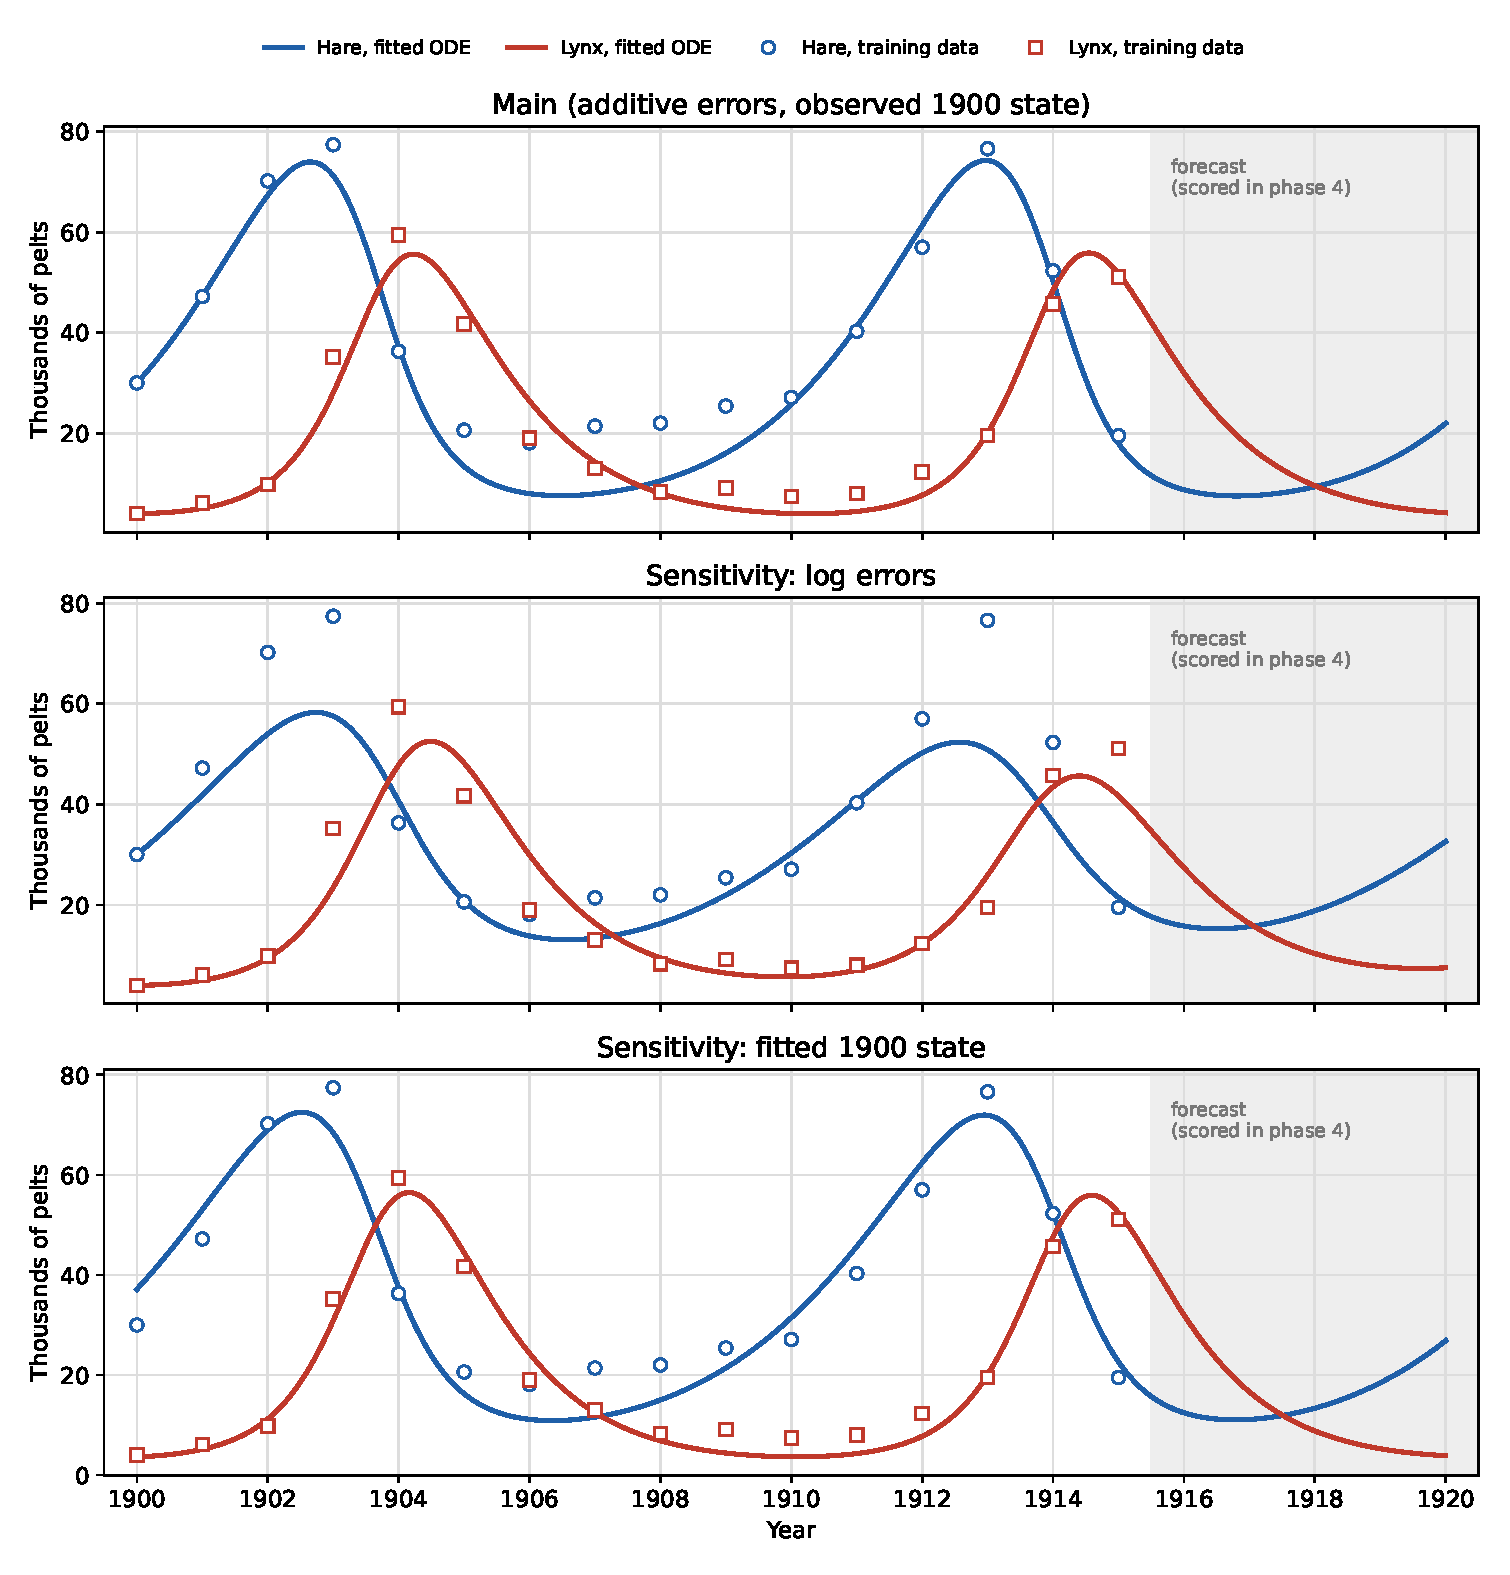
\includegraphics[width=0.9\textwidth]{advay_baseline_fit}
\caption{Least-squares fits to the 1900--1915 pelt counts (markers) and their continuation
through 1920 (shaded, held out) for the main analysis and both sensitivity variants.}
\label{fig:advay-fit}
\end{figure}

\begin{figure}[ht]
\centering
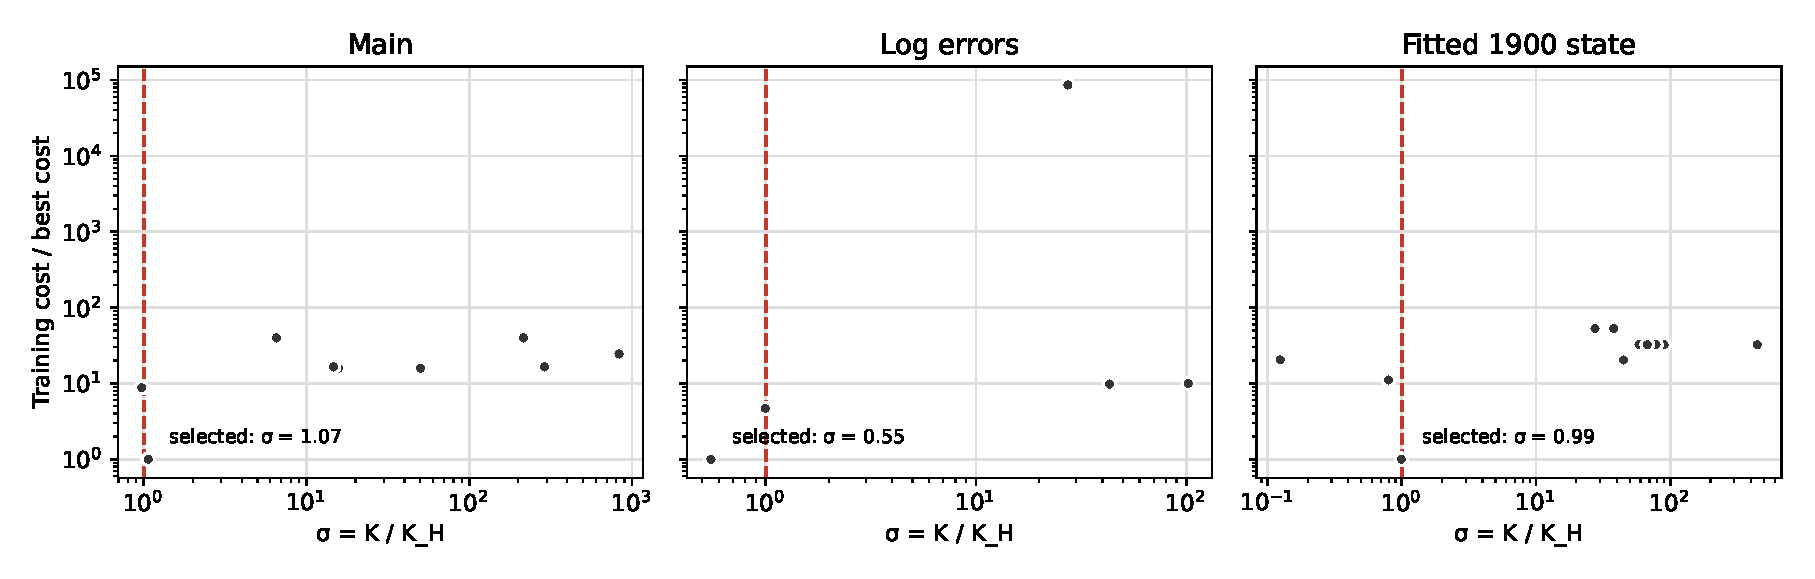
\includegraphics[width=\textwidth]{advay_baseline_sigma}
\caption{Training cost relative to the best, against $\sigma=K/K_H$, for every converged
start. The dashed line is the Hopf threshold $\sigma=1$. The best fits sit near $\sigma=1$,
on different sides depending on the variant.}\label{fig:advay-sigma}
\end{figure}

\subsection{Held-out evaluation, 1916--1920}\label{sec:advay-eval}

\paragraph{Protocol.} A scoring plan fixing the forecasts compared, the headline comparison,
the metrics and the interpretation rule was committed and published before the test file was
opened. All forecasts integrate frozen parameters from 1900 through 1920 with the shared
solver; nothing restarts from a test value, and no neural-network extrapolation is used.
For each species separately we report
$\mathrm{RMSE}=\big(\tfrac15\sum(\hat Y-Y)^2\big)^{1/2}$ and
$\mathrm{MAE}=\tfrac15\sum|\hat Y-Y|$ in thousands of pelts. With five test points a method
is called \emph{better} only if both its RMSE and MAE are smaller \emph{and} it is closer in
at least three of the five years; otherwise the methods are \emph{similar}. Two reference
forecasts use training data only: the 1915 value held constant (persistence) and the
1900--1915 mean. The headline comparison is the main least-squares fit against the
PINN-derived ODE forecast of the historical PINN study (seed chosen by training loss
before scoring). Every frozen forecast was checksum-verified, and the scores reproduce the
PINN study's own evaluation exactly.

\begin{table}[ht]
\centering
\input{tables/advay_heldout_metrics}
\caption{Held-out errors, 1916--1920, thousands of pelts.}\label{tab:advay-metrics}
\end{table}

\paragraph{Results.} (Table~\ref{tab:advay-metrics}, Figures~\ref{fig:advay-overlay}
and~\ref{fig:advay-metrics}.)
\begin{itemize}
\item \textbf{Both methods forecast the crash and recovery.} In the main variant both predict
the 1916--1920 lynx collapse and the hare recovery to within about 3--4 thousand pelts, far
better than persistence (lynx RMSE 37.2) or the training mean (lynx 10.6, hare 25.9). The
fitted dynamics carry real information about the next half-cycle.
\item \textbf{Headline: mixed and close.} Hare: similar (RMSE 3.07 least squares,
2.85 PINN; MAE 2.59 both). Lynx: least squares better (3.04 against 4.32, closer in all five
years); the PINN-derived lynx forecast falls to 3--5 thousand after 1918 where 9.7--10.1 were
observed.
\item \textbf{Sensitivity variants.} Least squares is better or similar in both. The log-error
PINN fit places the 1913 peaks about a year early and its forecast errors are large (hare RMSE 18.4).
\item \textbf{Why they differ.} Evaluated on $C$, the selected PINN parameters fit the
training years 1.9--3.4 times worse than the least-squares optimum, as expected for an
estimator that minimises a combined data and physics loss, and they cycle more strongly
($\sigma\approx1.35$). A better training fit did not give a better hare forecast in the main
variant. With five points, none of these differences is strong evidence.
\end{itemize}

\begin{figure}[ht]
\centering
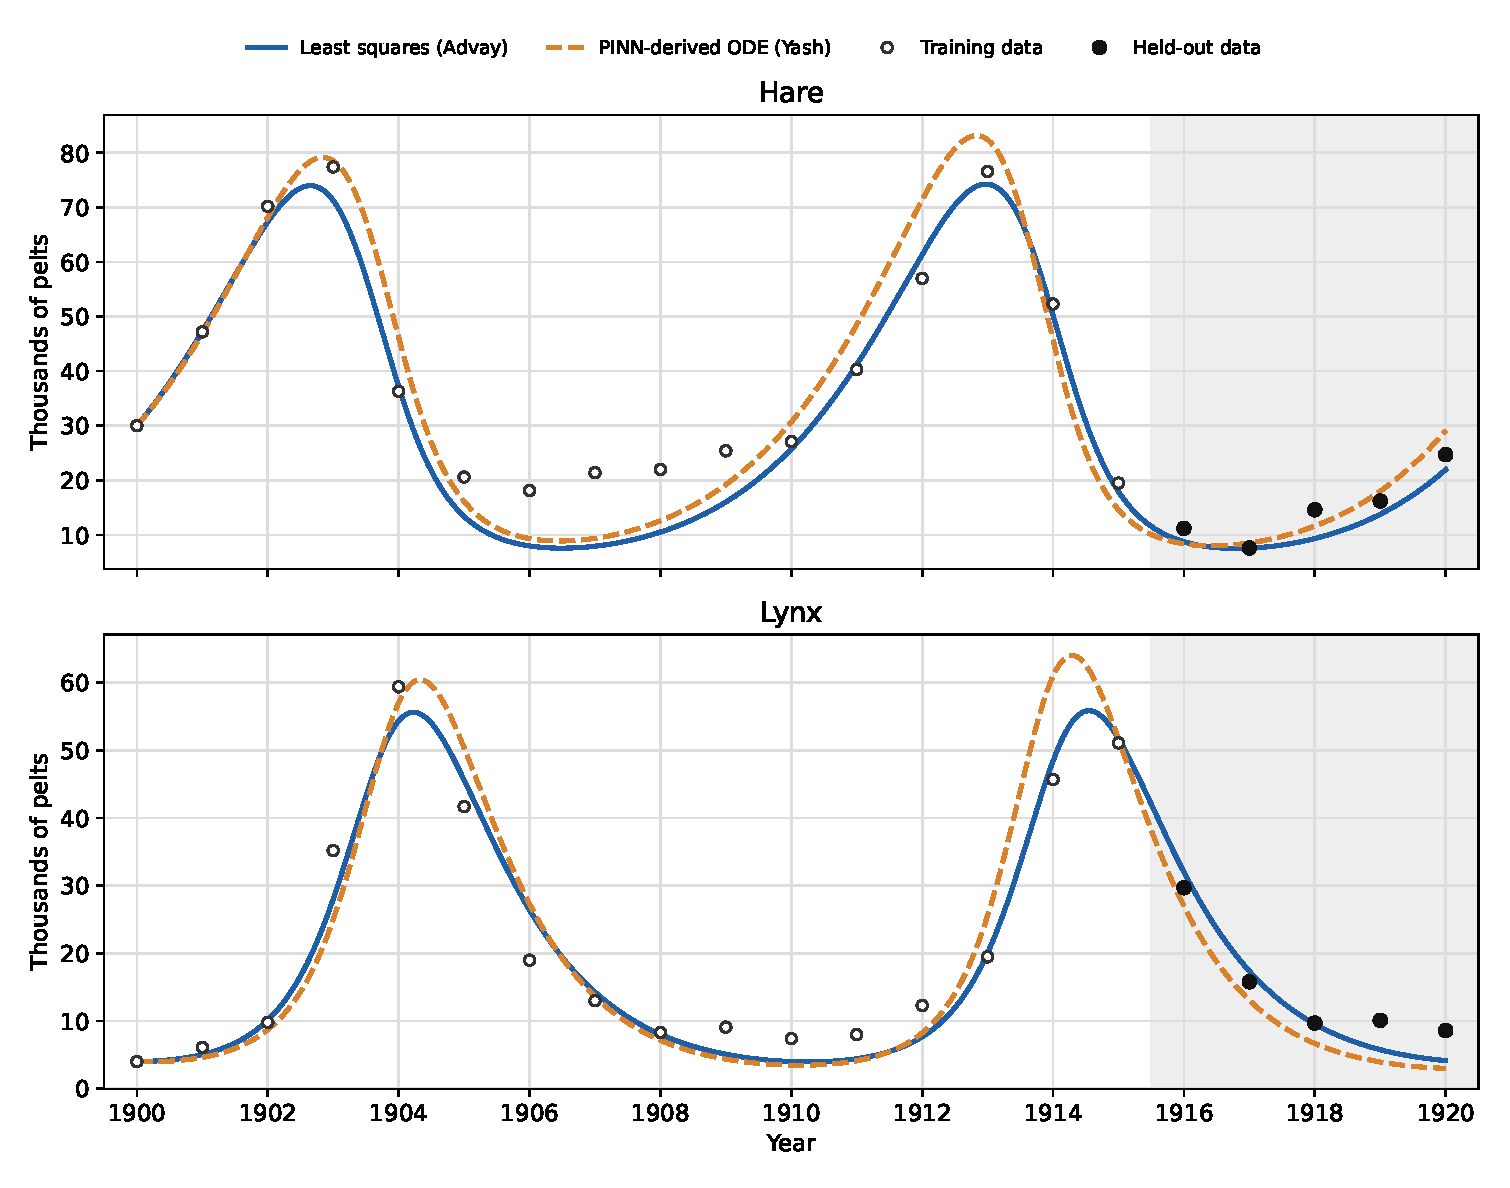
\includegraphics[width=0.9\textwidth]{advay_heldout_overlay}
\caption{Least-squares (solid) and PINN-derived (dashed) fits, main variant. Open circles:
training data; filled circles: held-out data (shaded). Both were fitted to 1900--1915 only
and integrated forward from 1900.}\label{fig:advay-overlay}
\end{figure}

\begin{figure}[ht]
\centering
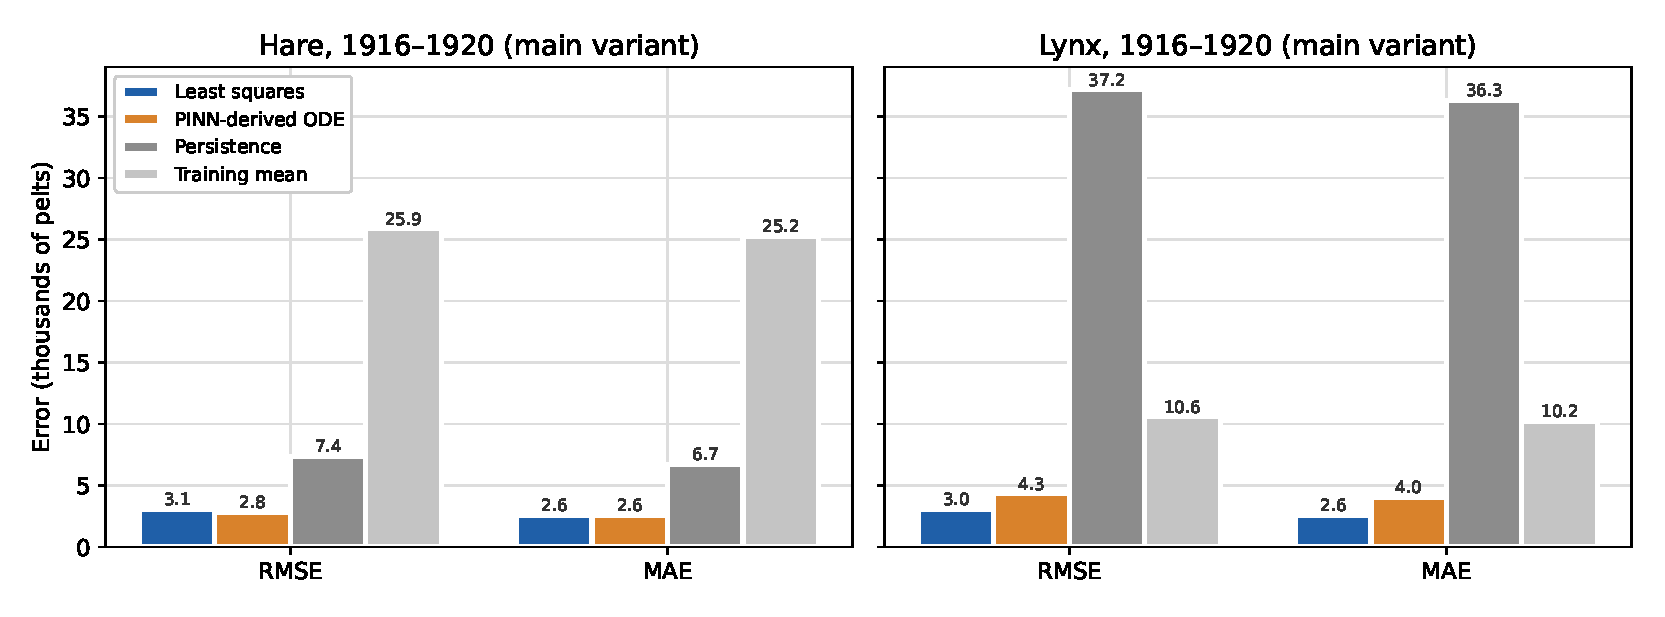
\includegraphics[width=\textwidth]{advay_heldout_metrics}
\caption{Held-out RMSE and MAE, main variant, with the persistence and training-mean
reference forecasts.}\label{fig:advay-metrics}
\end{figure}

\subsection{Limitations}\label{sec:advay-limits}

\begin{itemize}
\item \textbf{A very small test.} Five annual points, about half a cycle, beginning at the
1915 lynx peak. The comparison measures one crash and recovery, not long-run accuracy.
\item \textbf{Trade counts, not populations.} O1 assumes constant catchability; trapping
effort, prices and lynx behaviour almost certainly varied. Annual totals are treated as
point samples, a mismatch of up to a year in timing.
\item \textbf{Source uncertainty.} Two compilations of the same records disagree by more than
the forecast errors in some years; all results are conditional on the Stan series.
\item \textbf{Initial state.} The main analysis treats the noisy 1900 counts as exact. Fitting
them instead moves $\sigma$ from 1.07 to 0.99 and lowers the hare error.
\item \textbf{Identifiability.} $K$, $a$ and $b$ are individually poorly determined and $b$
(and $a$ in the main fit) lies on the box boundary, so their values depend on the chosen
bounds. A good curve fit is not evidence of uniquely recovered biological rates.
\item \textbf{Observation model.} Changing only the error model (additive to log) changes
$\sigma$ from 1.07 to 0.55 and the hare/lynx error balance, so the qualitative dynamics
inferred are sensitive to how the counts are assumed to be measured.
\item \textbf{Missing ecology.} A closed two-species, constant-parameter model omits
vegetation, other predators, weather, disease and spatial structure. Its success over
1916--1920 shows that it captures the dominant short-term feedback, not that it is complete.
\end{itemize}

\paragraph{Reproduction.} \texttt{scripts/advay\_data\_checks.py},
\texttt{advay\_make\_split.py}, \texttt{advay\_fit\_baseline.py --protocol v2},
\texttt{advay\_compare\_benchmark.py} and \texttt{advay\_score\_heldout.py} regenerate every
number and figure in this section; the declared protocols are in
\texttt{docs/advay\_baseline\_protocol.md} and \texttt{docs/advay\_scoring\_plan.md}.
   (standalone build: advay_main.tex)
% Figures: graphs/advay_*.{eps,pdf}; table: tables/advay_heldout_metrics.tex.
\section{Data, Least-Squares Baseline and Validation}\label{sec:advay}

This section states what the historical observations are, how they were prepared, how the
model was fitted to them by nonlinear least squares, and how well the fitted model forecasts
years it never saw. Every analysis choice that could be influenced by the held-out years was
written down and committed to the project repository before those years were opened.

\subsection{Data source and meaning}\label{sec:advay-data}

We use annual counts of snowshoe hare and Canadian lynx pelts traded by the Hudson's Bay
Company, 1900--1920, in thousands of pelts, as distributed with the Stan case study
\cite{carpenter2018}. Carpenter traces the numbers through Howard's lecture notes
\cite{howard2009} to a biology textbook; the original source is the Company's fur returns,
discussed by Hewitt \cite{hewitt1921}. The values are used unchanged
(\texttt{data/historical/pelts\_1900\_1920.csv}); the file's provenance, checksums and every
transformation (removing comment lines, reordering columns) are recorded alongside it.

These are \emph{trade counts}, not censuses. Trapping effort, fur prices, the number of
reporting posts and animal behaviour all affect them; Hewitt notes that hungry lynx are
easier to trap when hares are scarce. A second widely used compilation, the tsibbledata
\texttt{pelt} series \cite{tsibbledata_pelt}, differs noticeably over the same years
(Figure~\ref{fig:advay-sources}): the correlation between the two is 0.81 for lynx but only
0.32 for hare, and individual hare values differ by more than our forecast errors. We use
the Stan series because the project protocol names it, and treat the disagreement as a source
of uncertainty that no model in this report can remove.

\begin{figure}[ht]
\centering
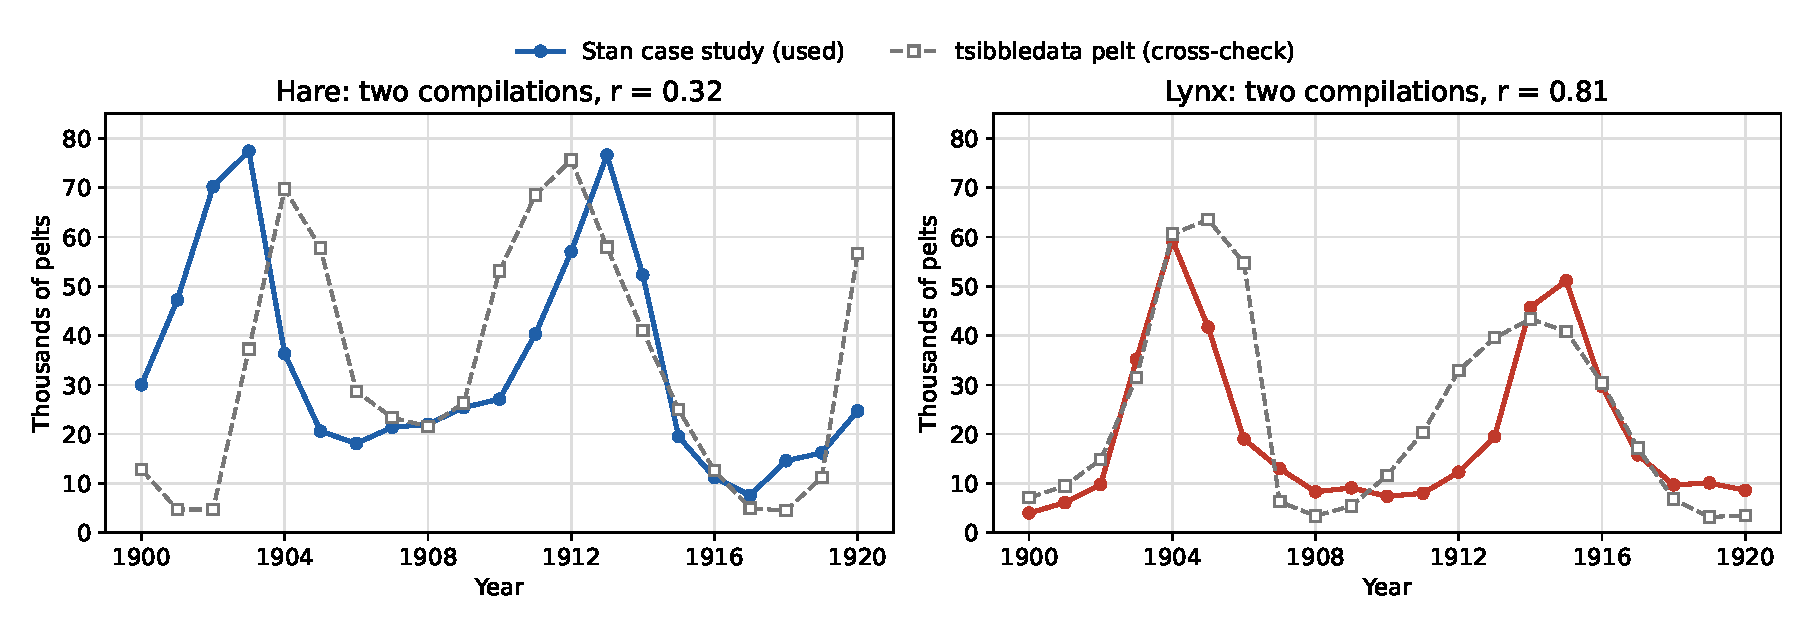
\includegraphics[width=\textwidth]{advay_source_comparison}
\caption{The Stan case-study series used here (solid) and the tsibbledata \texttt{pelt}
compilation (dashed) for 1900--1920. Both show two cycles, but yearly values differ,
especially for hare.}\label{fig:advay-sources}
\end{figure}

\paragraph{Observation model.} Following the agreed convention (assumption O1), pelt counts
are taken to be proportional to animal numbers with unknown constant factors, and the model
states are defined directly in pelt units:
\[
Y_{H,i}=H(t_i)+\varepsilon_{H,i},\qquad Y_{P,i}=P(t_i)+\varepsilon_{P,i},\qquad t_i=\mathrm{Year}_i-1900,
\]
with each annual total treated as a sample of the state at $t_i$. No observation scale factor
is fitted. Under O1, $r$, $m$ and the dimensionless groups of the model section are unchanged
by the unknown factors; $K$, $b$, $a$ and $e$ are \emph{effective} coefficients in pelt
units and are not interpreted as absolute biological quantities.

\subsection{Preparation and exploratory checks}\label{sec:advay-checks}

The 21 rows are consecutive, with no missing values, no zeros and no duplicates. The data
were split once into a training file (1900--1915, 16 rows) and a test file (1916--1920,
5 rows), with checksums recorded; all fitting code reads only the training file. Every
statistic below uses the training years only.

\begin{itemize}
\item \textbf{Cycles and lag.} Hare peaks in 1903 and 1913 (a ten-year spacing); lynx peaks
in 1904 and at the 1915 boundary. The correlation of $H(t)$ with $P(t+k)$ is largest at
$k=2$ years ($r=0.94$; $0.76$ at $k=1$). In the hare--lynx plane the data trace
counter-clockwise loops, as predator--prey models predict (Figure~\ref{fig:advay-raw}).
\item \textbf{Outliers.} None: robust $z$-scores of year-to-year log growth stay below 3
(largest 2.94, the 1903--1904 hare crash).
\item \textbf{Scale.} Training ranges are 18.1--77.4 (hare) and 4.0--59.4 (lynx). Hare counts
are about twice lynx counts, so residuals are divided by each species' training maximum
$(s_H,s_P)=(77.4,59.4)$ to weight the species equally. No log transform is used in the main
analysis; a log-residual fit is a declared sensitivity check.
\item \textbf{Split position.} Training ends exactly at the 1915 lynx peak, so the test years
are the following crash and the start of recovery: a turning point the fit never sees in
that cycle.
\end{itemize}

\begin{figure}[ht]
\centering
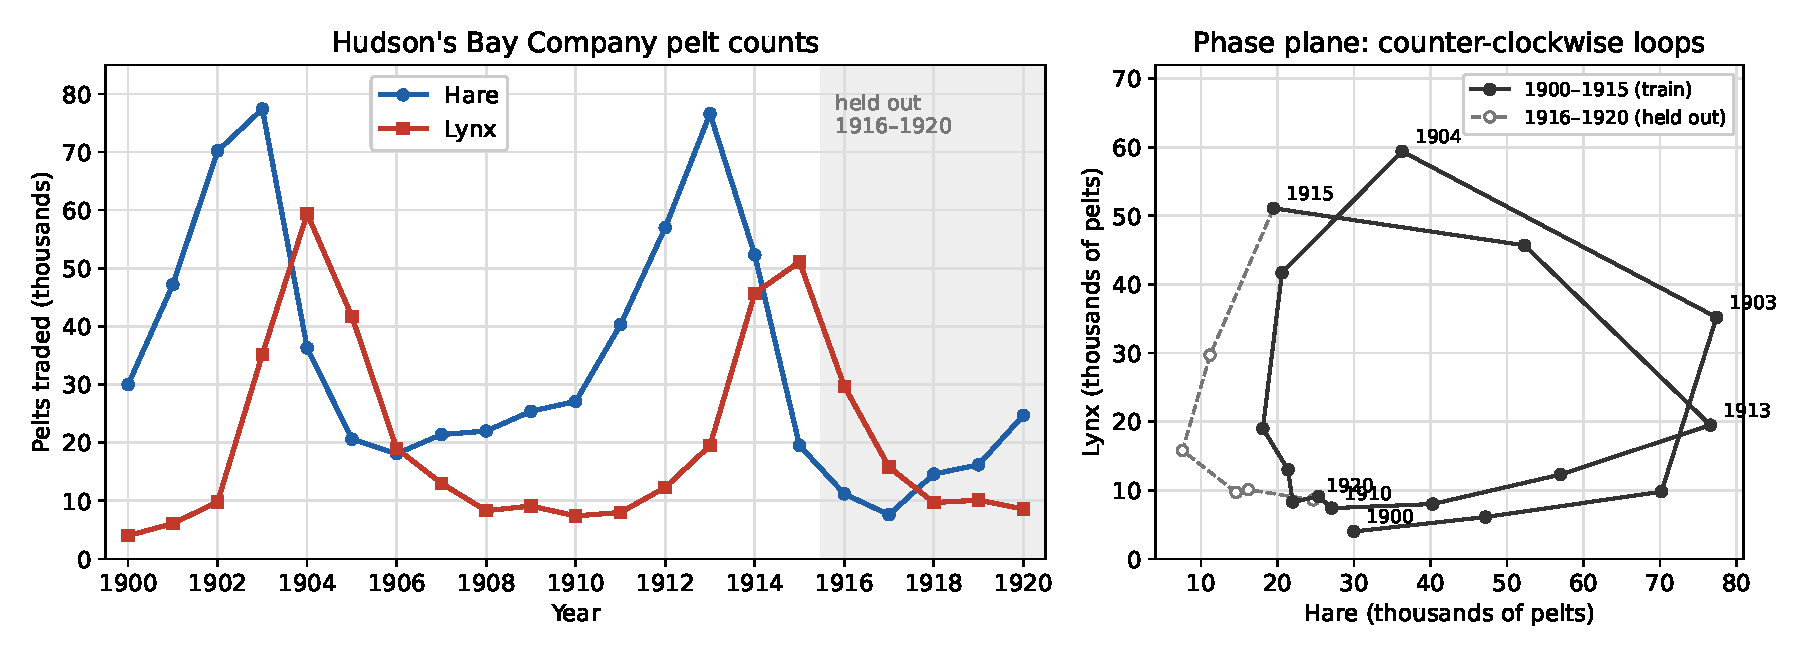
\includegraphics[width=\textwidth]{advay_raw_series}
\caption{Left: annual pelt counts, 1900--1920; the shaded band is held out. Right: the same
data in the hare--lynx plane (training solid, held-out dashed).}\label{fig:advay-raw}
\end{figure}

\subsection{Least-squares baseline}\label{sec:advay-ls}

\paragraph{Problem.} With $\theta=(r,K,a,b,e,m)$ and the shared RK45 solver (relative
tolerance $10^{-8}$, absolute $10^{-10}$, maximum step $0.1$ years), let $\hat H(t;\theta)$,
$\hat P(t;\theta)$ solve the model from the observed 1900 state $(30.0,4.0)$. The main
estimate minimises
\[
C(\theta)=\tfrac12\sum_{i=1900}^{1915}\Big[\big(\tfrac{\hat H(t_i;\theta)-Y_{H,i}}{s_H}\big)^2+
\big(\tfrac{\hat P(t_i;\theta)-Y_{P,i}}{s_P}\big)^2\Big]
\]
over the shared box bounds $r,m\in[0.05,3]$, $K\in[20,500]$, $a\in[0.05,10]$,
$b\in[0.5,300]$, $e\in[0.02,5]$. Two declared sensitivity variants change one assumption
each: \emph{log errors} replaces the scaled residuals by $\log\hat Y-\log Y$, and
\emph{fitted 1900 state} adds $(H_0,P_0)$ as unknowns within $[0.5,1.5]$ times the observed
values.

\paragraph{Method.} The bounded trust-region reflective algorithm (SciPy
\texttt{least\_squares}) is run in log-parameter space $x=\log\theta$, because the bounds
span up to a 600-fold range. Finite-difference steps of $10^{-4}$ in $x$ stay well above the
solver tolerance. The objective is multimodal, so each variant uses 80 starts: the shared
initial guess, 39 Latin-hypercube points uniform in $\log\theta$ and 39 uniform in $\theta$.
The fit with the lowest training cost is selected.

\paragraph{Protocol record.} The settings were committed before the first run. That run
(40 log-space starts) missed the best \emph{fitted 1900 state} fit, which an independent
benchmark had found at training cost $0.063$ against our $0.70$; evaluating our objective at
the benchmark's parameters gave $0.063$, so the code agreed and the start design was at
fault (the optimum sits near the upper bounds, which log-uniform starts rarely visit). The
uniform-scale starts were added as a declared amendment, judged on training cost alone and
before any test score of the baseline was computed. Both runs are kept.

\begin{table}[ht]
\centering
\begin{tabular}{lrrrrrrrl}
\toprule
Variant & $C$ & $r$ & $K$ & $a$ & $b$ & $e$ & $m$ & $\sigma=K/K_H$\\
\midrule
Main & 0.0845 & 0.647 & 382 & 10.0$^*$ & 300$^*$ & 0.967 & 0.857 & 1.07 (cycle)\\
Log errors & 0.903 & 0.520 & 197 & 7.17 & 300$^*$ & 1.80 & 1.15 & 0.55 (damped)\\
Fitted 1900 state & 0.0634 & 0.520 & 362 & 8.15 & 300$^*$ & 1.32 & 1.05 & 0.99 (damped)\\
\bottomrule
\end{tabular}
\caption{Least-squares estimates. $^*$ at the upper bound. Units: $r,m$ per year; $K,b$
thousands of hare pelts; $a,e$ effective pelt-unit coefficients. The fitted 1900 state in the
last variant is $(37.1,3.64)$.}\label{tab:advay-ls}
\end{table}

\paragraph{Results.} Table~\ref{tab:advay-ls} and Figure~\ref{fig:advay-fit} give the selected
fits. Three findings matter for interpretation.
\begin{enumerate}
\item \emph{The optimum is computationally well defined.} In every variant all starts within
1\% of the best cost (18, 42 and 16 of 80) found the same parameters to four significant
figures, and a separately written least-squares code by another team member reaches the same
optimum (training costs within $2\times10^{-7}$, forecasts within 0.002 thousand pelts).
\item \emph{The saturation of predation is not identified.} $b$ sits on its upper bound in
every variant. With $b$ about four times the largest hare count, $aH/(b+H)\approx(a/b)H$ over
the data: predation is nearly linear in hare abundance. In the linearised fit the
correlation between $\log a$ and $\log b$ is 0.998 and the approximate standard errors of
$\log K$, $\log a$, $\log b$ exceed 1 (a factor of three or more), whereas $r$, $e$, $m$ are
determined to about 10--40\%. Only the ratio $a/b\approx0.024$--$0.033$ is well determined.
Because the optimum lies on the boundary, its location depends on the chosen box.
\item \emph{Limit cycle or damped oscillation is not decided.} Using the Hopf threshold
$K_H=b(ea+m)/(ea-m)$ from the stability analysis, $\sigma$ is 1.07 for the main fit (just past the threshold),
0.99 with a fitted 1900 state (just below) and 0.55 with log errors. All three reproduce the
observed timing equally well (hare peaks fitted at 1902.5--1902.8 and 1912.6--1913.0, lynx
1.6 years later, period about ten years). Two cycles of data cannot distinguish a stable
limit cycle from a slowly damped oscillation (Figure~\ref{fig:advay-sigma}).
\end{enumerate}

\begin{figure}[ht]
\centering
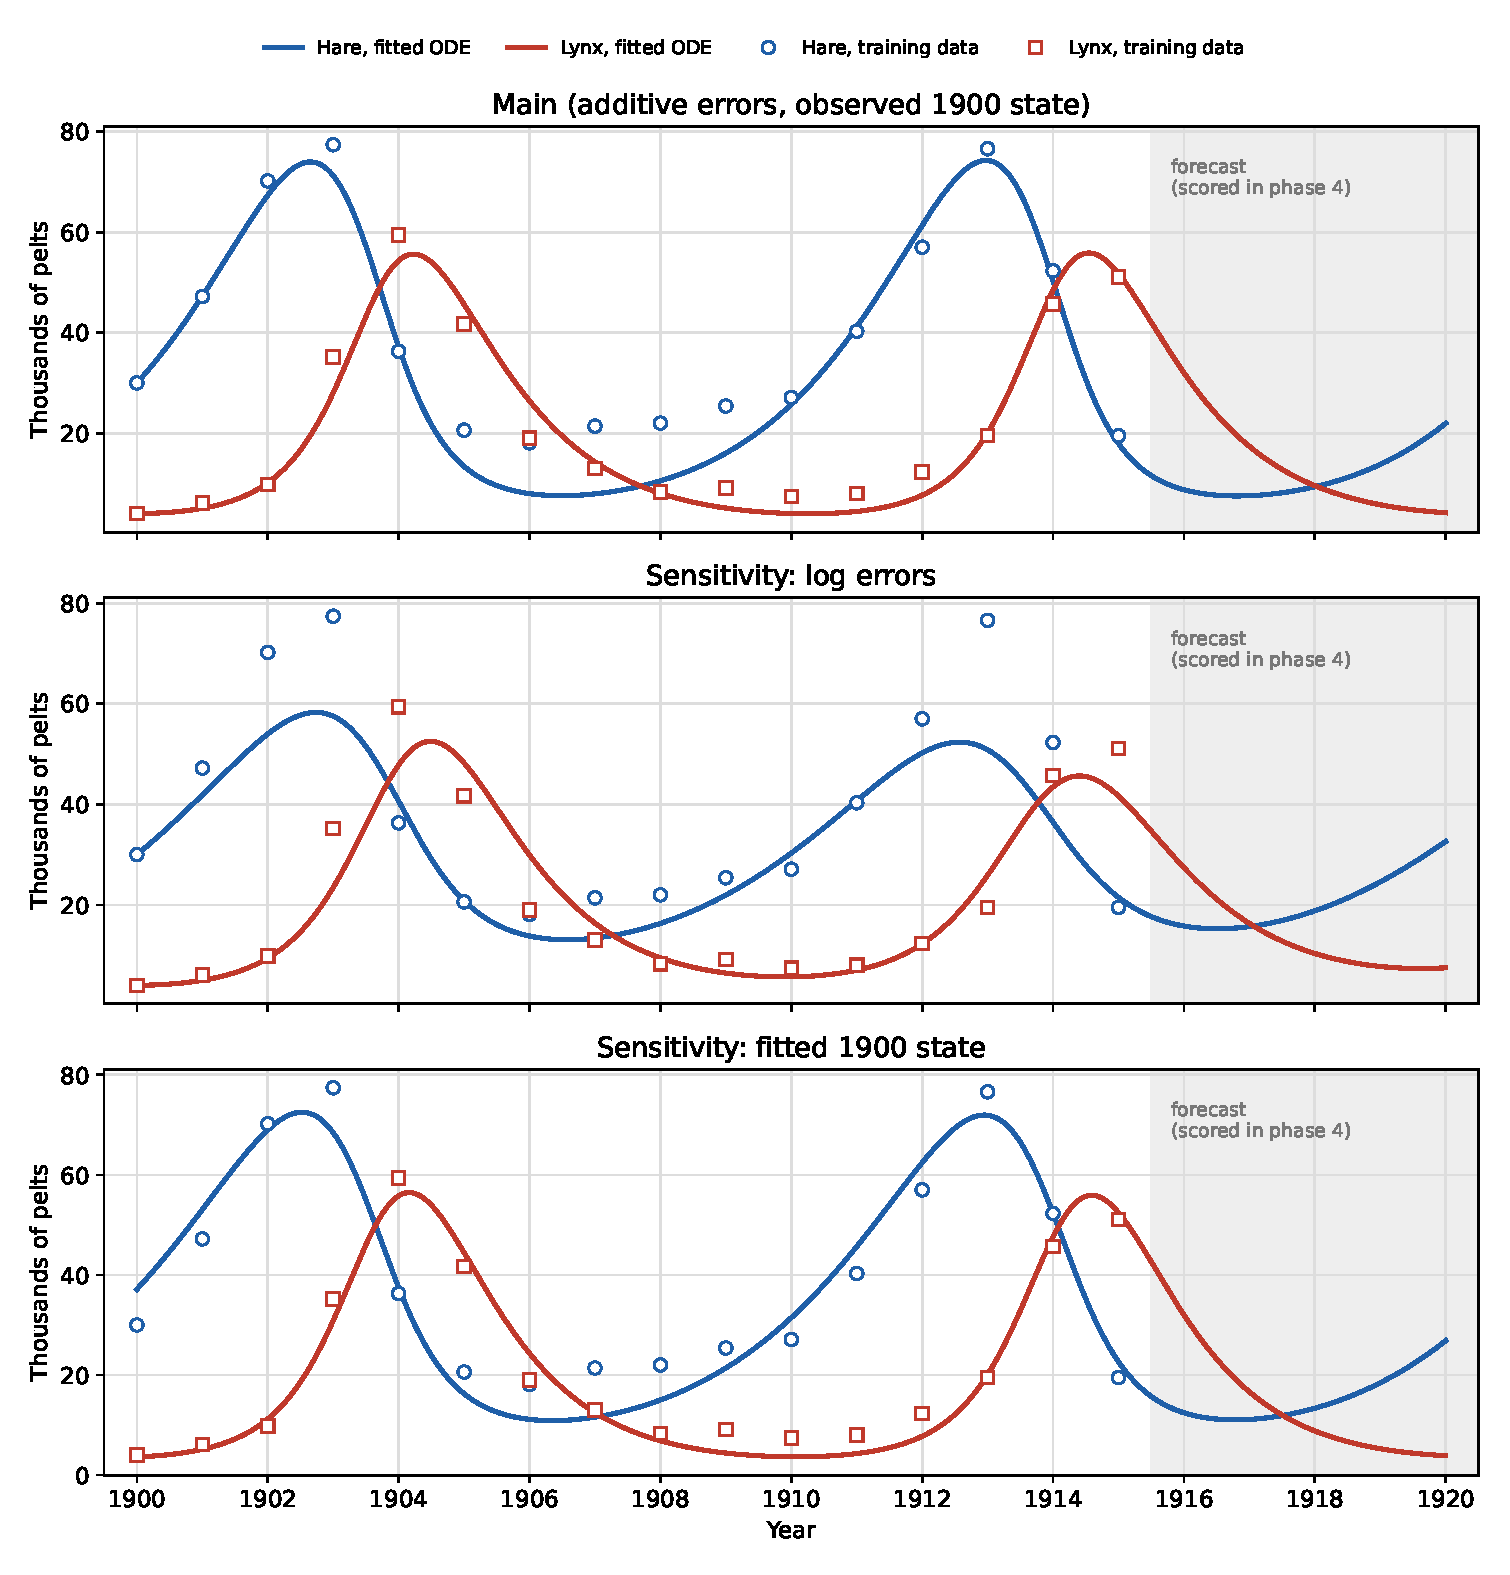
\includegraphics[width=0.9\textwidth]{advay_baseline_fit}
\caption{Least-squares fits to the 1900--1915 pelt counts (markers) and their continuation
through 1920 (shaded, held out) for the main analysis and both sensitivity variants.}
\label{fig:advay-fit}
\end{figure}

\begin{figure}[ht]
\centering
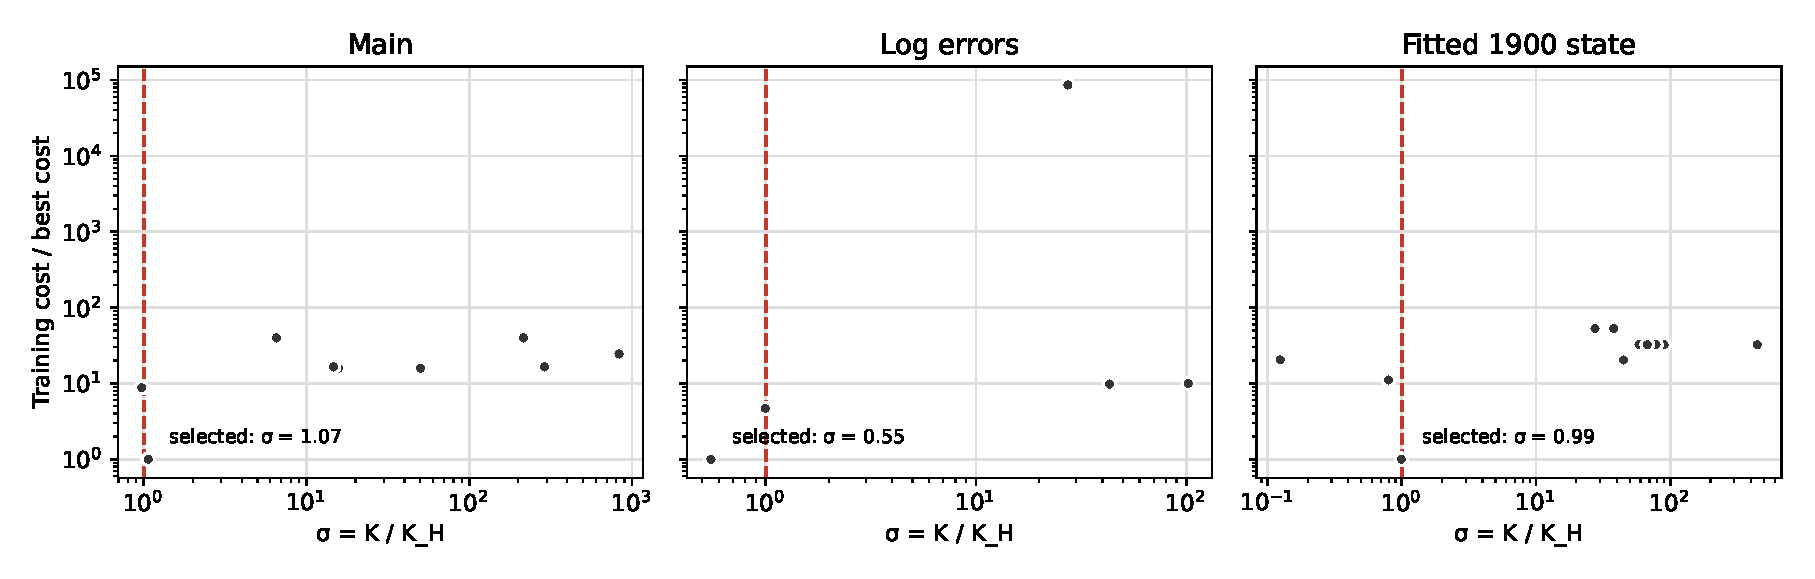
\includegraphics[width=\textwidth]{advay_baseline_sigma}
\caption{Training cost relative to the best, against $\sigma=K/K_H$, for every converged
start. The dashed line is the Hopf threshold $\sigma=1$. The best fits sit near $\sigma=1$,
on different sides depending on the variant.}\label{fig:advay-sigma}
\end{figure}

\subsection{Held-out evaluation, 1916--1920}\label{sec:advay-eval}

\paragraph{Protocol.} A scoring plan fixing the forecasts compared, the headline comparison,
the metrics and the interpretation rule was committed and published before the test file was
opened. All forecasts integrate frozen parameters from 1900 through 1920 with the shared
solver; nothing restarts from a test value, and no neural-network extrapolation is used.
For each species separately we report
$\mathrm{RMSE}=\big(\tfrac15\sum(\hat Y-Y)^2\big)^{1/2}$ and
$\mathrm{MAE}=\tfrac15\sum|\hat Y-Y|$ in thousands of pelts. With five test points a method
is called \emph{better} only if both its RMSE and MAE are smaller \emph{and} it is closer in
at least three of the five years; otherwise the methods are \emph{similar}. Two reference
forecasts use training data only: the 1915 value held constant (persistence) and the
1900--1915 mean. The headline comparison is the main least-squares fit against the
PINN-derived ODE forecast of the historical PINN study (seed chosen by training loss
before scoring). Every frozen forecast was checksum-verified, and the scores reproduce the
PINN study's own evaluation exactly.

\begin{table}[ht]
\centering
\begin{tabular}{llrrrr}
\hline
Variant & Method & Hare RMSE & Hare MAE & Lynx RMSE & Lynx MAE \\
\hline
Main (headline) & Least squares & 3.07 & 2.59 & 3.04 & 2.56 \\
 & PINN-derived ODE (seed17) & 2.85 & 2.59 & 4.32 & 4.05 \\
Log errors & Least squares & 6.87 & 6.63 & 1.60 & 1.38 \\
 & PINN-derived ODE (seed29) & 18.35 & 14.29 & 10.03 & 8.97 \\
Fitted 1900 state & Least squares & 2.25 & 2.08 & 3.24 & 2.71 \\
 & PINN-derived ODE (seed17) & 3.69 & 3.06 & 4.70 & 4.53 \\
\hline
Reference & Persistence (1915 value) & 7.38 & 6.72 & 37.16 & 36.32 \\
Reference & Training mean & 25.87 & 25.23 & 10.58 & 10.21 \\
\hline
\end{tabular}

\caption{Held-out errors, 1916--1920, thousands of pelts.}\label{tab:advay-metrics}
\end{table}

\paragraph{Results.} (Table~\ref{tab:advay-metrics}, Figures~\ref{fig:advay-overlay}
and~\ref{fig:advay-metrics}.)
\begin{itemize}
\item \textbf{Both methods forecast the crash and recovery.} In the main variant both predict
the 1916--1920 lynx collapse and the hare recovery to within about 3--4 thousand pelts, far
better than persistence (lynx RMSE 37.2) or the training mean (lynx 10.6, hare 25.9). The
fitted dynamics carry real information about the next half-cycle.
\item \textbf{Headline: mixed and close.} Hare: similar (RMSE 3.07 least squares,
2.85 PINN; MAE 2.59 both). Lynx: least squares better (3.04 against 4.32, closer in all five
years); the PINN-derived lynx forecast falls to 3--5 thousand after 1918 where 9.7--10.1 were
observed.
\item \textbf{Sensitivity variants.} Least squares is better or similar in both. The log-error
PINN fit places the 1913 peaks about a year early and its forecast errors are large (hare RMSE 18.4).
\item \textbf{Why they differ.} Evaluated on $C$, the selected PINN parameters fit the
training years 1.9--3.4 times worse than the least-squares optimum, as expected for an
estimator that minimises a combined data and physics loss, and they cycle more strongly
($\sigma\approx1.35$). A better training fit did not give a better hare forecast in the main
variant. With five points, none of these differences is strong evidence.
\end{itemize}

\begin{figure}[ht]
\centering
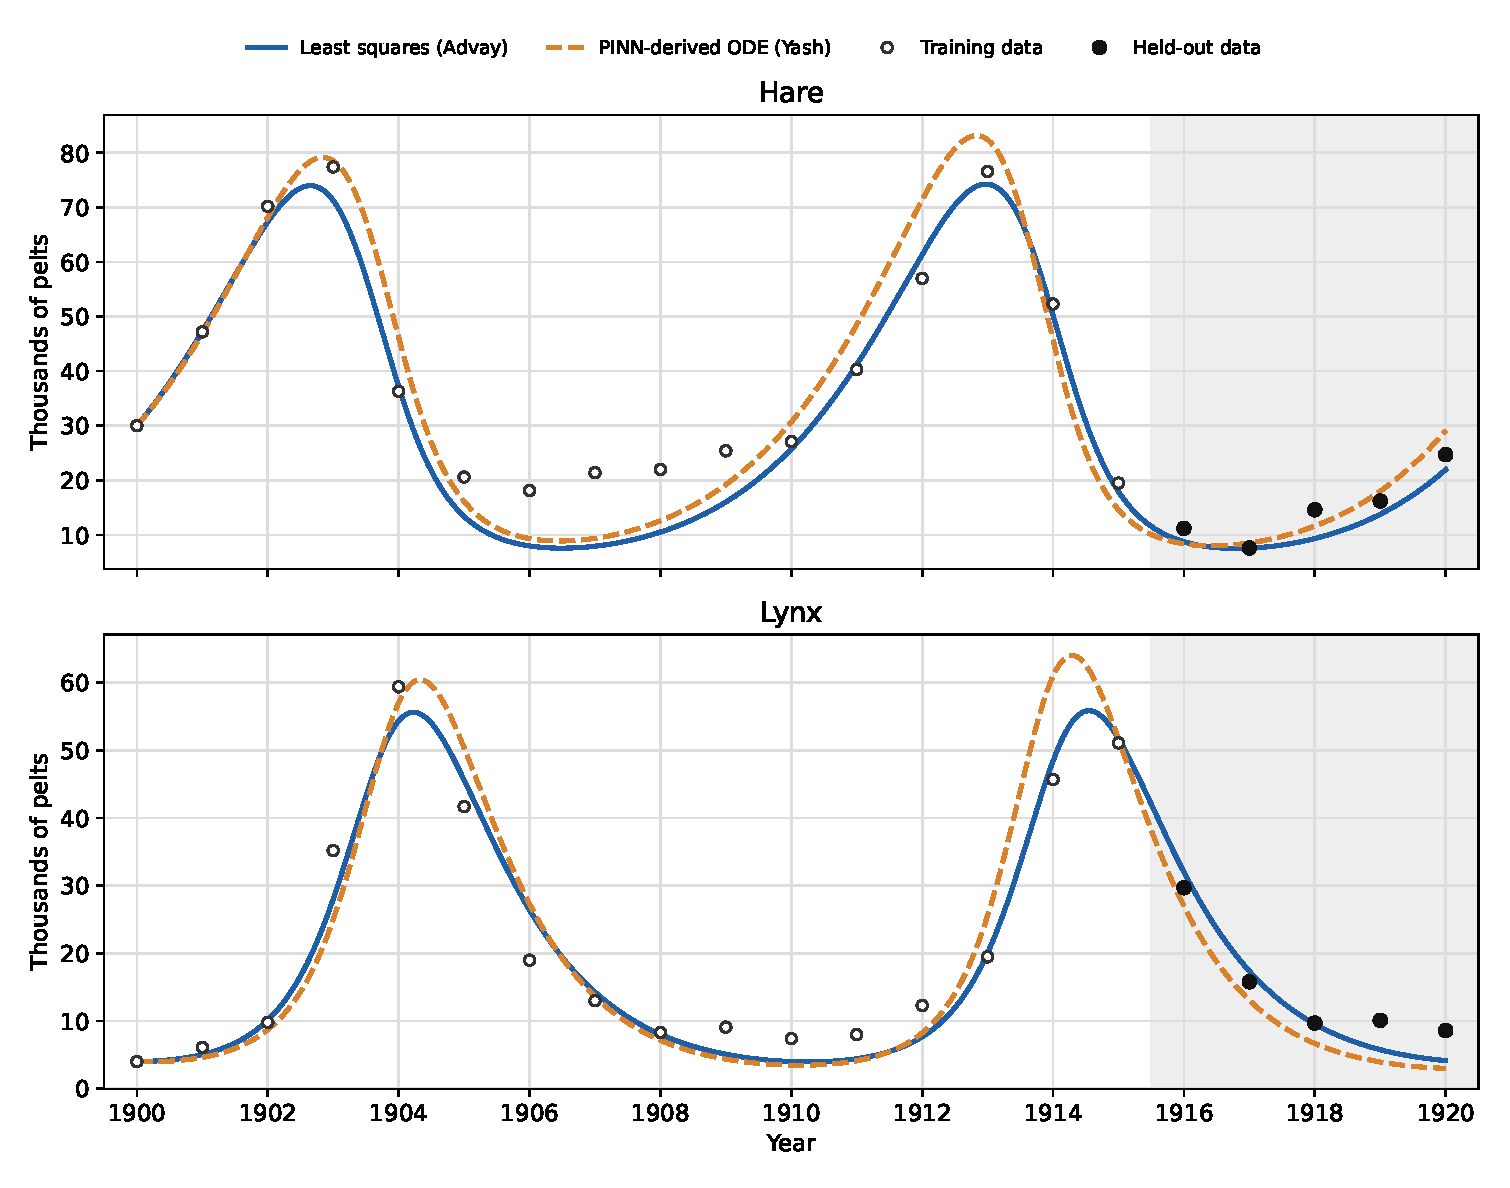
\includegraphics[width=0.9\textwidth]{advay_heldout_overlay}
\caption{Least-squares (solid) and PINN-derived (dashed) fits, main variant. Open circles:
training data; filled circles: held-out data (shaded). Both were fitted to 1900--1915 only
and integrated forward from 1900.}\label{fig:advay-overlay}
\end{figure}

\begin{figure}[ht]
\centering
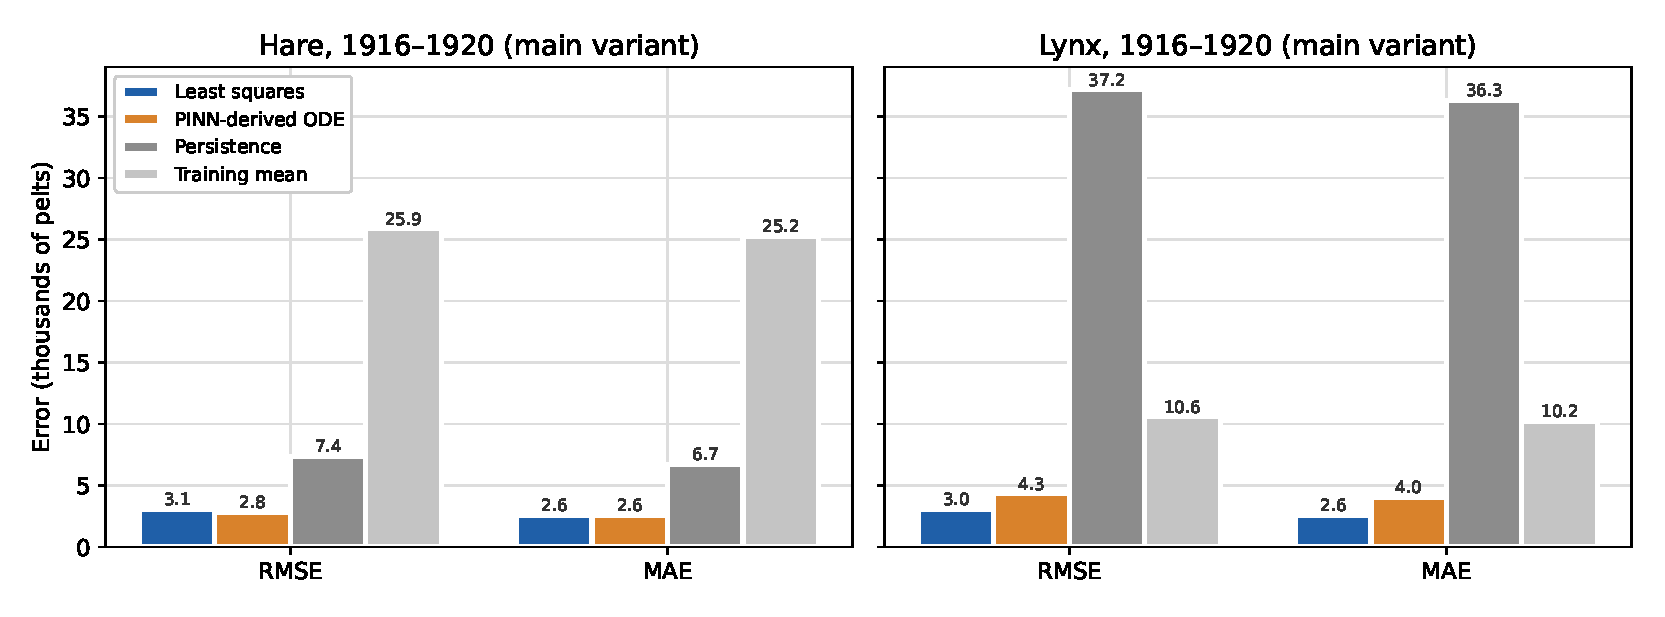
\includegraphics[width=\textwidth]{advay_heldout_metrics}
\caption{Held-out RMSE and MAE, main variant, with the persistence and training-mean
reference forecasts.}\label{fig:advay-metrics}
\end{figure}

\subsection{Limitations}\label{sec:advay-limits}

\begin{itemize}
\item \textbf{A very small test.} Five annual points, about half a cycle, beginning at the
1915 lynx peak. The comparison measures one crash and recovery, not long-run accuracy.
\item \textbf{Trade counts, not populations.} O1 assumes constant catchability; trapping
effort, prices and lynx behaviour almost certainly varied. Annual totals are treated as
point samples, a mismatch of up to a year in timing.
\item \textbf{Source uncertainty.} Two compilations of the same records disagree by more than
the forecast errors in some years; all results are conditional on the Stan series.
\item \textbf{Initial state.} The main analysis treats the noisy 1900 counts as exact. Fitting
them instead moves $\sigma$ from 1.07 to 0.99 and lowers the hare error.
\item \textbf{Identifiability.} $K$, $a$ and $b$ are individually poorly determined and $b$
(and $a$ in the main fit) lies on the box boundary, so their values depend on the chosen
bounds. A good curve fit is not evidence of uniquely recovered biological rates.
\item \textbf{Observation model.} Changing only the error model (additive to log) changes
$\sigma$ from 1.07 to 0.55 and the hare/lynx error balance, so the qualitative dynamics
inferred are sensitive to how the counts are assumed to be measured.
\item \textbf{Missing ecology.} A closed two-species, constant-parameter model omits
vegetation, other predators, weather, disease and spatial structure. Its success over
1916--1920 shows that it captures the dominant short-term feedback, not that it is complete.
\end{itemize}

\paragraph{Reproduction.} \texttt{scripts/advay\_data\_checks.py},
\texttt{advay\_make\_split.py}, \texttt{advay\_fit\_baseline.py --protocol v2},
\texttt{advay\_compare\_benchmark.py} and \texttt{advay\_score\_heldout.py} regenerate every
number and figure in this section; the declared protocols are in
\texttt{docs/advay\_baseline\_protocol.md} and \texttt{docs/advay\_scoring\_plan.md}.
   (standalone build: advay_main.tex)
% Figures: graphs/advay_*.{eps,pdf}; table: tables/advay_heldout_metrics.tex.
\section{Data, Least-Squares Baseline and Validation}\label{sec:advay}

This section states what the historical observations are, how they were prepared, how the
model was fitted to them by nonlinear least squares, and how well the fitted model forecasts
years it never saw. Every analysis choice that could be influenced by the held-out years was
written down and committed to the project repository before those years were opened.

\subsection{Data source and meaning}\label{sec:advay-data}

We use annual counts of snowshoe hare and Canadian lynx pelts traded by the Hudson's Bay
Company, 1900--1920, in thousands of pelts, as distributed with the Stan case study
\cite{carpenter2018}. Carpenter traces the numbers through Howard's lecture notes
\cite{howard2009} to a biology textbook; the original source is the Company's fur returns,
discussed by Hewitt \cite{hewitt1921}. The values are used unchanged
(\texttt{data/historical/pelts\_1900\_1920.csv}); the file's provenance, checksums and every
transformation (removing comment lines, reordering columns) are recorded alongside it.

These are \emph{trade counts}, not censuses. Trapping effort, fur prices, the number of
reporting posts and animal behaviour all affect them; Hewitt notes that hungry lynx are
easier to trap when hares are scarce. A second widely used compilation, the tsibbledata
\texttt{pelt} series \cite{tsibbledata_pelt}, differs noticeably over the same years
(Figure~\ref{fig:advay-sources}): the correlation between the two is 0.81 for lynx but only
0.32 for hare, and individual hare values differ by more than our forecast errors. We use
the Stan series because the project protocol names it, and treat the disagreement as a source
of uncertainty that no model in this report can remove.

\begin{figure}[ht]
\centering
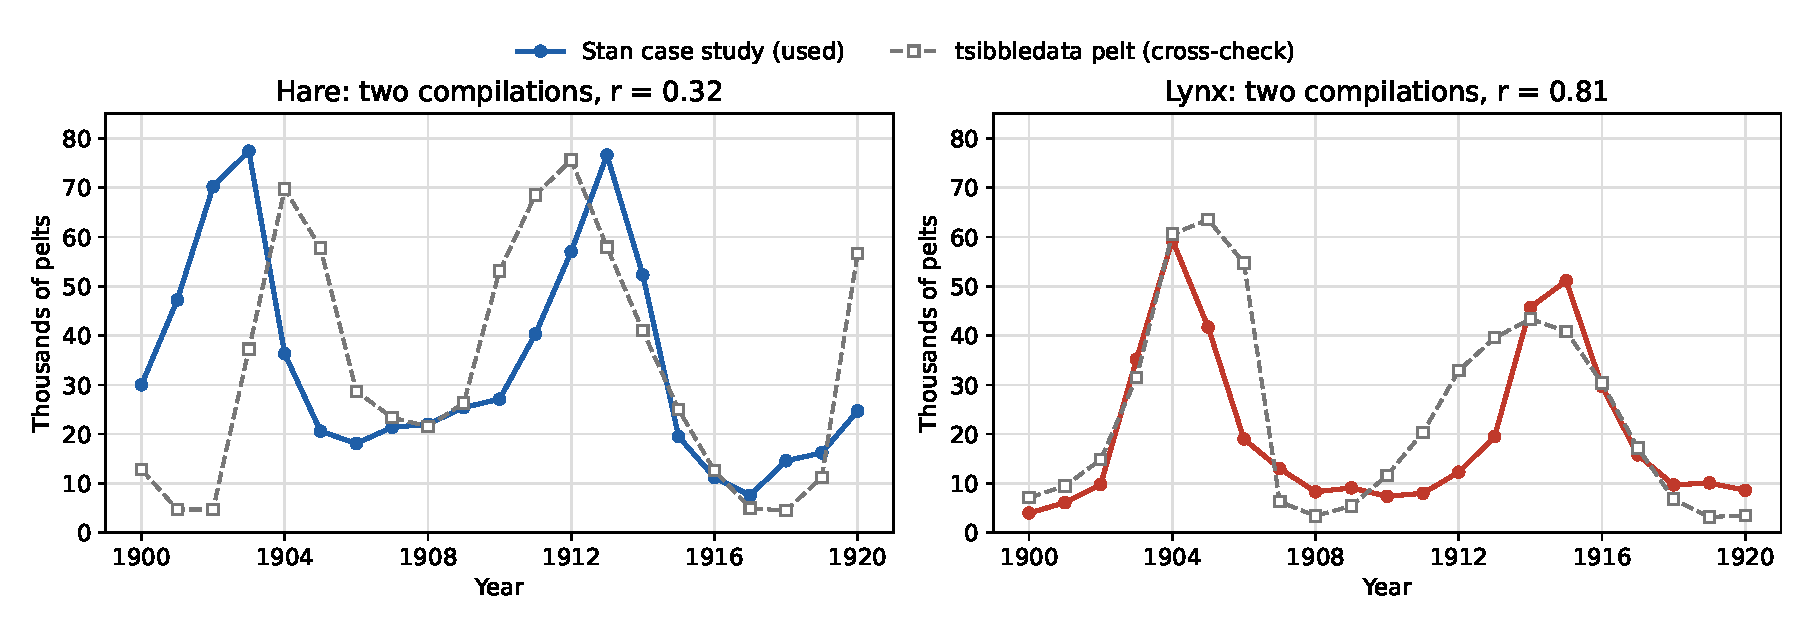
\includegraphics[width=\textwidth]{advay_source_comparison}
\caption{The Stan case-study series used here (solid) and the tsibbledata \texttt{pelt}
compilation (dashed) for 1900--1920. Both show two cycles, but yearly values differ,
especially for hare.}\label{fig:advay-sources}
\end{figure}

\paragraph{Observation model.} Following the agreed convention (assumption O1), pelt counts
are taken to be proportional to animal numbers with unknown constant factors, and the model
states are defined directly in pelt units:
\[
Y_{H,i}=H(t_i)+\varepsilon_{H,i},\qquad Y_{P,i}=P(t_i)+\varepsilon_{P,i},\qquad t_i=\mathrm{Year}_i-1900,
\]
with each annual total treated as a sample of the state at $t_i$. No observation scale factor
is fitted. Under O1, $r$, $m$ and the dimensionless groups of the model section are unchanged
by the unknown factors; $K$, $b$, $a$ and $e$ are \emph{effective} coefficients in pelt
units and are not interpreted as absolute biological quantities.

\subsection{Preparation and exploratory checks}\label{sec:advay-checks}

The 21 rows are consecutive, with no missing values, no zeros and no duplicates. The data
were split once into a training file (1900--1915, 16 rows) and a test file (1916--1920,
5 rows), with checksums recorded; all fitting code reads only the training file. Every
statistic below uses the training years only.

\begin{itemize}
\item \textbf{Cycles and lag.} Hare peaks in 1903 and 1913 (a ten-year spacing); lynx peaks
in 1904 and at the 1915 boundary. The correlation of $H(t)$ with $P(t+k)$ is largest at
$k=2$ years ($r=0.94$; $0.76$ at $k=1$). In the hare--lynx plane the data trace
counter-clockwise loops, as predator--prey models predict (Figure~\ref{fig:advay-raw}).
\item \textbf{Outliers.} None: robust $z$-scores of year-to-year log growth stay below 3
(largest 2.94, the 1903--1904 hare crash).
\item \textbf{Scale.} Training ranges are 18.1--77.4 (hare) and 4.0--59.4 (lynx). Hare counts
are about twice lynx counts, so residuals are divided by each species' training maximum
$(s_H,s_P)=(77.4,59.4)$ to weight the species equally. No log transform is used in the main
analysis; a log-residual fit is a declared sensitivity check.
\item \textbf{Split position.} Training ends exactly at the 1915 lynx peak, so the test years
are the following crash and the start of recovery: a turning point the fit never sees in
that cycle.
\end{itemize}

\begin{figure}[ht]
\centering
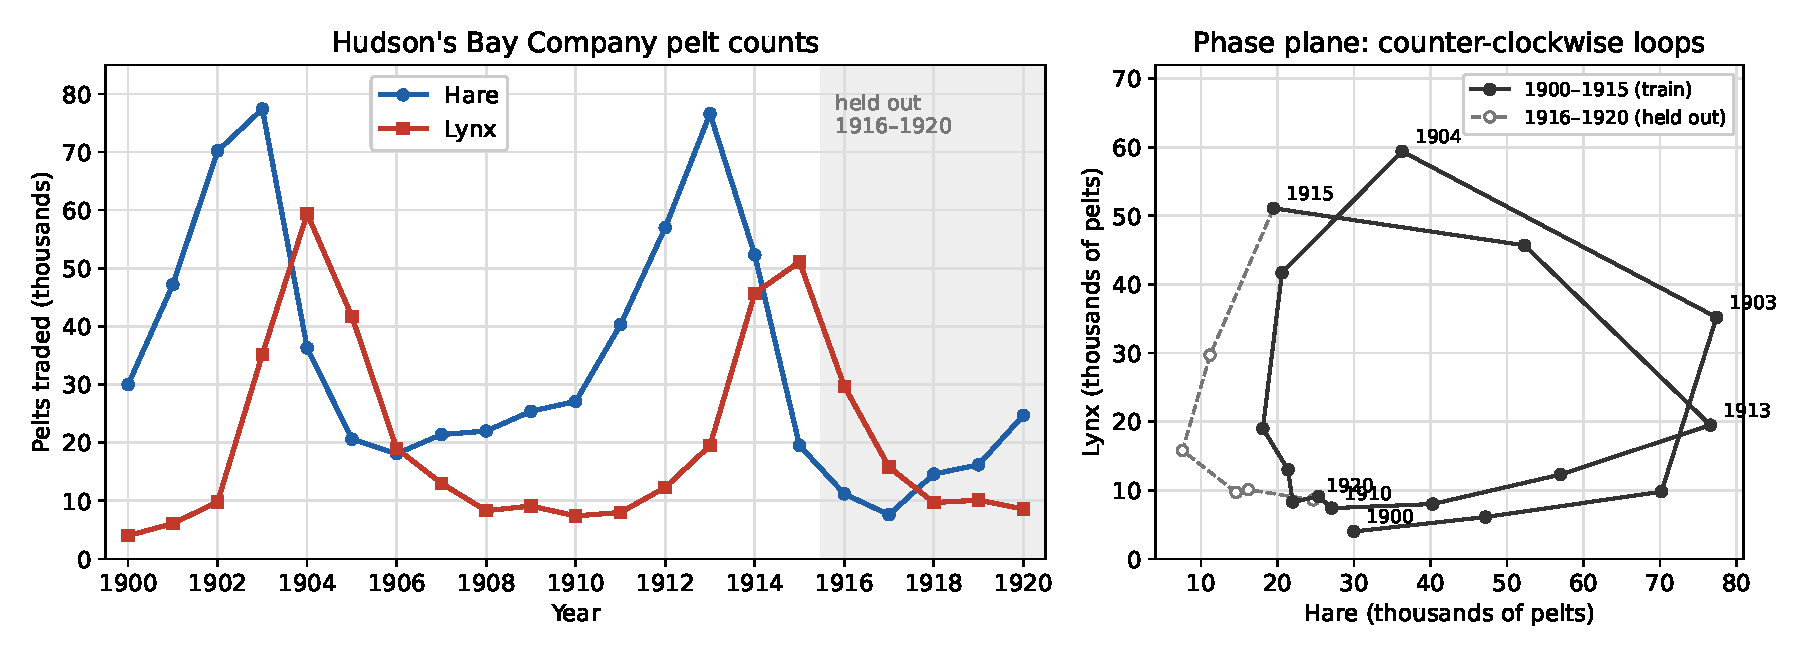
\includegraphics[width=\textwidth]{advay_raw_series}
\caption{Left: annual pelt counts, 1900--1920; the shaded band is held out. Right: the same
data in the hare--lynx plane (training solid, held-out dashed).}\label{fig:advay-raw}
\end{figure}

\subsection{Least-squares baseline}\label{sec:advay-ls}

\paragraph{Problem.} With $\theta=(r,K,a,b,e,m)$ and the shared RK45 solver (relative
tolerance $10^{-8}$, absolute $10^{-10}$, maximum step $0.1$ years), let $\hat H(t;\theta)$,
$\hat P(t;\theta)$ solve the model from the observed 1900 state $(30.0,4.0)$. The main
estimate minimises
\[
C(\theta)=\tfrac12\sum_{i=1900}^{1915}\Big[\big(\tfrac{\hat H(t_i;\theta)-Y_{H,i}}{s_H}\big)^2+
\big(\tfrac{\hat P(t_i;\theta)-Y_{P,i}}{s_P}\big)^2\Big]
\]
over the shared box bounds $r,m\in[0.05,3]$, $K\in[20,500]$, $a\in[0.05,10]$,
$b\in[0.5,300]$, $e\in[0.02,5]$. Two declared sensitivity variants change one assumption
each: \emph{log errors} replaces the scaled residuals by $\log\hat Y-\log Y$, and
\emph{fitted 1900 state} adds $(H_0,P_0)$ as unknowns within $[0.5,1.5]$ times the observed
values.

\paragraph{Method.} The bounded trust-region reflective algorithm (SciPy
\texttt{least\_squares}) is run in log-parameter space $x=\log\theta$, because the bounds
span up to a 600-fold range. Finite-difference steps of $10^{-4}$ in $x$ stay well above the
solver tolerance. The objective is multimodal, so each variant uses 80 starts: the shared
initial guess, 39 Latin-hypercube points uniform in $\log\theta$ and 39 uniform in $\theta$.
The fit with the lowest training cost is selected.

\paragraph{Protocol record.} The settings were committed before the first run. That run
(40 log-space starts) missed the best \emph{fitted 1900 state} fit, which an independent
benchmark had found at training cost $0.063$ against our $0.70$; evaluating our objective at
the benchmark's parameters gave $0.063$, so the code agreed and the start design was at
fault (the optimum sits near the upper bounds, which log-uniform starts rarely visit). The
uniform-scale starts were added as a declared amendment, judged on training cost alone and
before any test score of the baseline was computed. Both runs are kept.

\begin{table}[ht]
\centering
\begin{tabular}{lrrrrrrrl}
\toprule
Variant & $C$ & $r$ & $K$ & $a$ & $b$ & $e$ & $m$ & $\sigma=K/K_H$\\
\midrule
Main & 0.0845 & 0.647 & 382 & 10.0$^*$ & 300$^*$ & 0.967 & 0.857 & 1.07 (cycle)\\
Log errors & 0.903 & 0.520 & 197 & 7.17 & 300$^*$ & 1.80 & 1.15 & 0.55 (damped)\\
Fitted 1900 state & 0.0634 & 0.520 & 362 & 8.15 & 300$^*$ & 1.32 & 1.05 & 0.99 (damped)\\
\bottomrule
\end{tabular}
\caption{Least-squares estimates. $^*$ at the upper bound. Units: $r,m$ per year; $K,b$
thousands of hare pelts; $a,e$ effective pelt-unit coefficients. The fitted 1900 state in the
last variant is $(37.1,3.64)$.}\label{tab:advay-ls}
\end{table}

\paragraph{Results.} Table~\ref{tab:advay-ls} and Figure~\ref{fig:advay-fit} give the selected
fits. Three findings matter for interpretation.
\begin{enumerate}
\item \emph{The optimum is computationally well defined.} In every variant all starts within
1\% of the best cost (18, 42 and 16 of 80) found the same parameters to four significant
figures, and a separately written least-squares code by another team member reaches the same
optimum (training costs within $2\times10^{-7}$, forecasts within 0.002 thousand pelts).
\item \emph{The saturation of predation is not identified.} $b$ sits on its upper bound in
every variant. With $b$ about four times the largest hare count, $aH/(b+H)\approx(a/b)H$ over
the data: predation is nearly linear in hare abundance. In the linearised fit the
correlation between $\log a$ and $\log b$ is 0.998 and the approximate standard errors of
$\log K$, $\log a$, $\log b$ exceed 1 (a factor of three or more), whereas $r$, $e$, $m$ are
determined to about 10--40\%. Only the ratio $a/b\approx0.024$--$0.033$ is well determined.
Because the optimum lies on the boundary, its location depends on the chosen box.
\item \emph{Limit cycle or damped oscillation is not decided.} Using the Hopf threshold
$K_H=b(ea+m)/(ea-m)$ from the stability analysis, $\sigma$ is 1.07 for the main fit (just past the threshold),
0.99 with a fitted 1900 state (just below) and 0.55 with log errors. All three reproduce the
observed timing equally well (hare peaks fitted at 1902.5--1902.8 and 1912.6--1913.0, lynx
1.6 years later, period about ten years). Two cycles of data cannot distinguish a stable
limit cycle from a slowly damped oscillation (Figure~\ref{fig:advay-sigma}).
\end{enumerate}

\begin{figure}[ht]
\centering
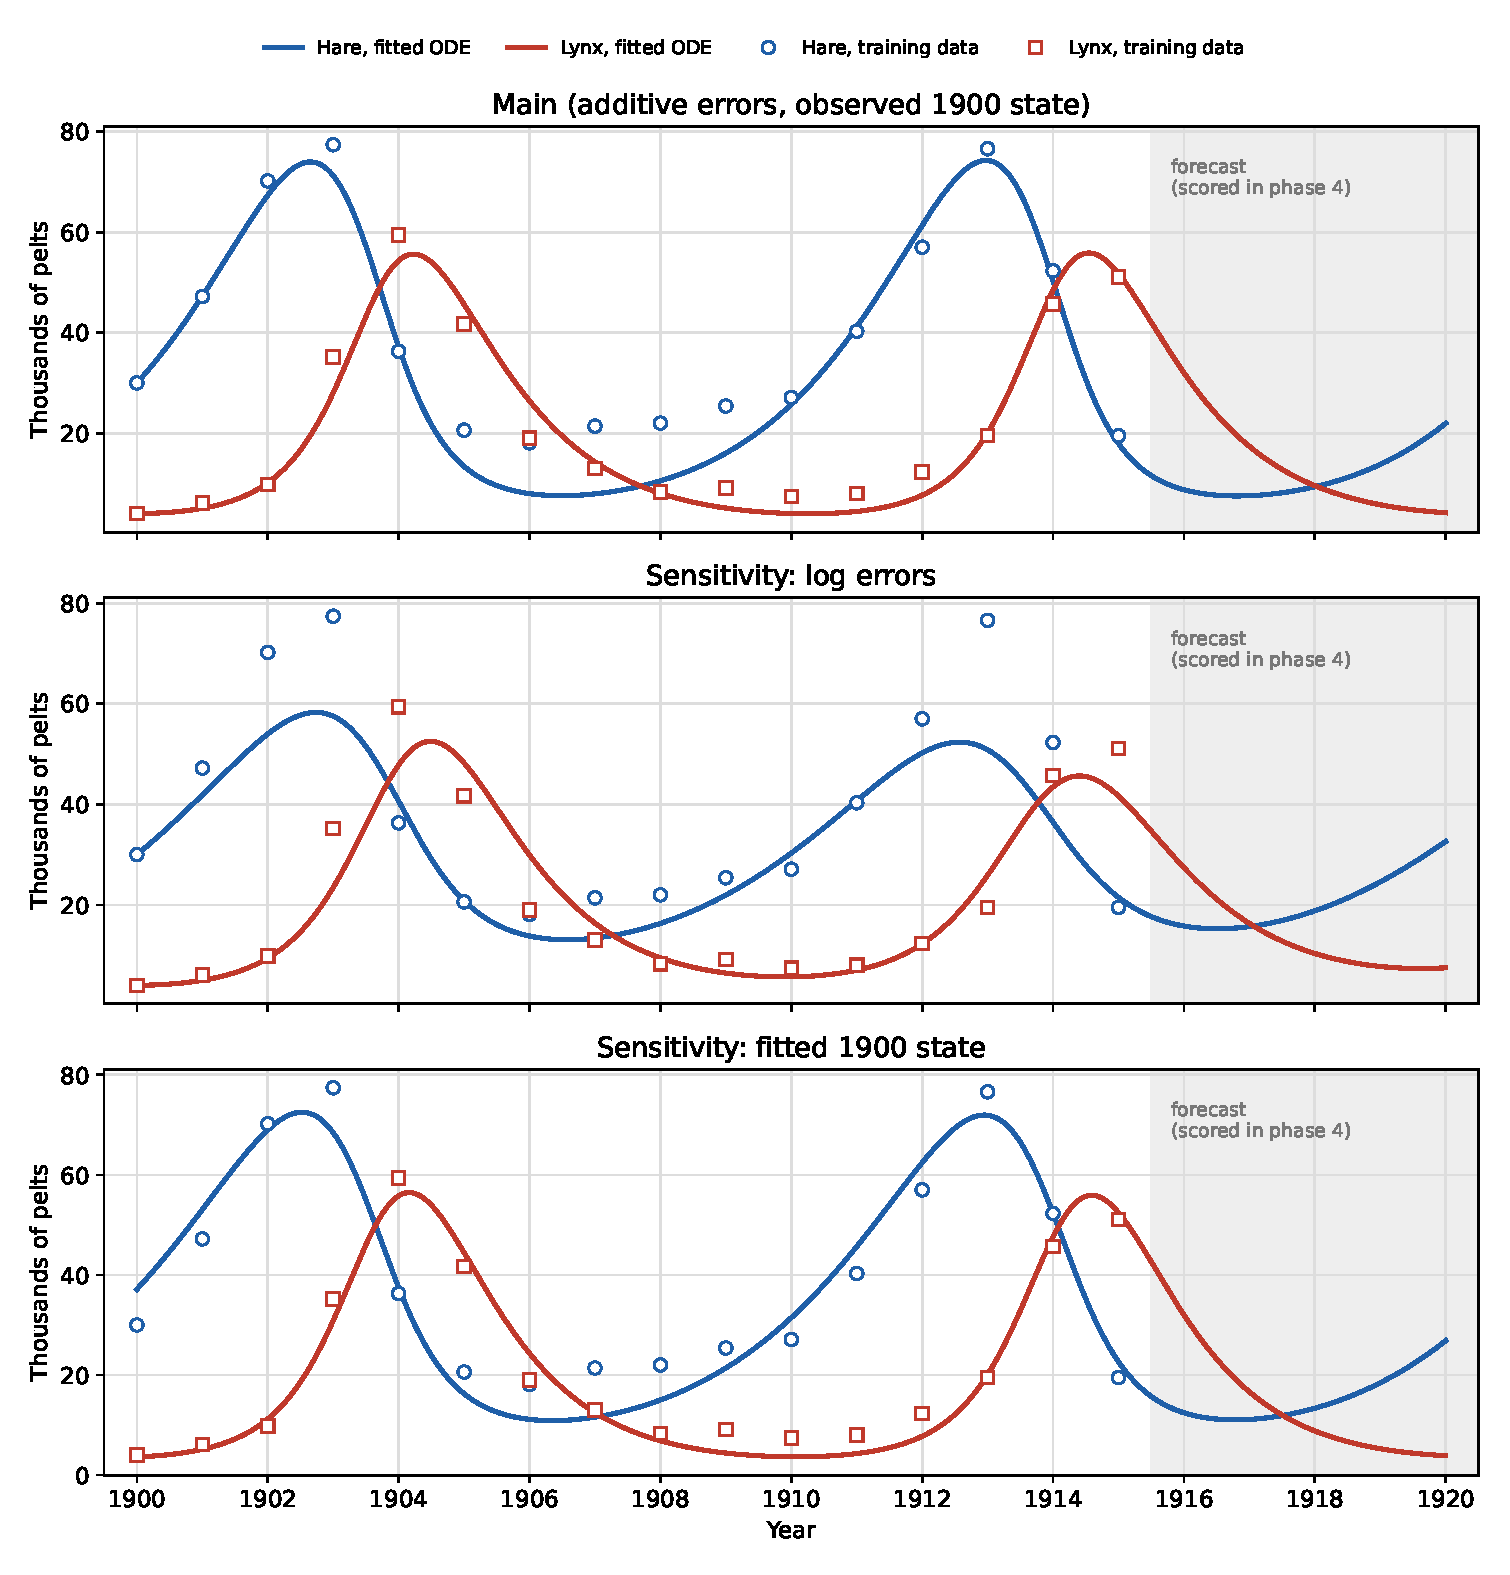
\includegraphics[width=0.9\textwidth]{advay_baseline_fit}
\caption{Least-squares fits to the 1900--1915 pelt counts (markers) and their continuation
through 1920 (shaded, held out) for the main analysis and both sensitivity variants.}
\label{fig:advay-fit}
\end{figure}

\begin{figure}[ht]
\centering
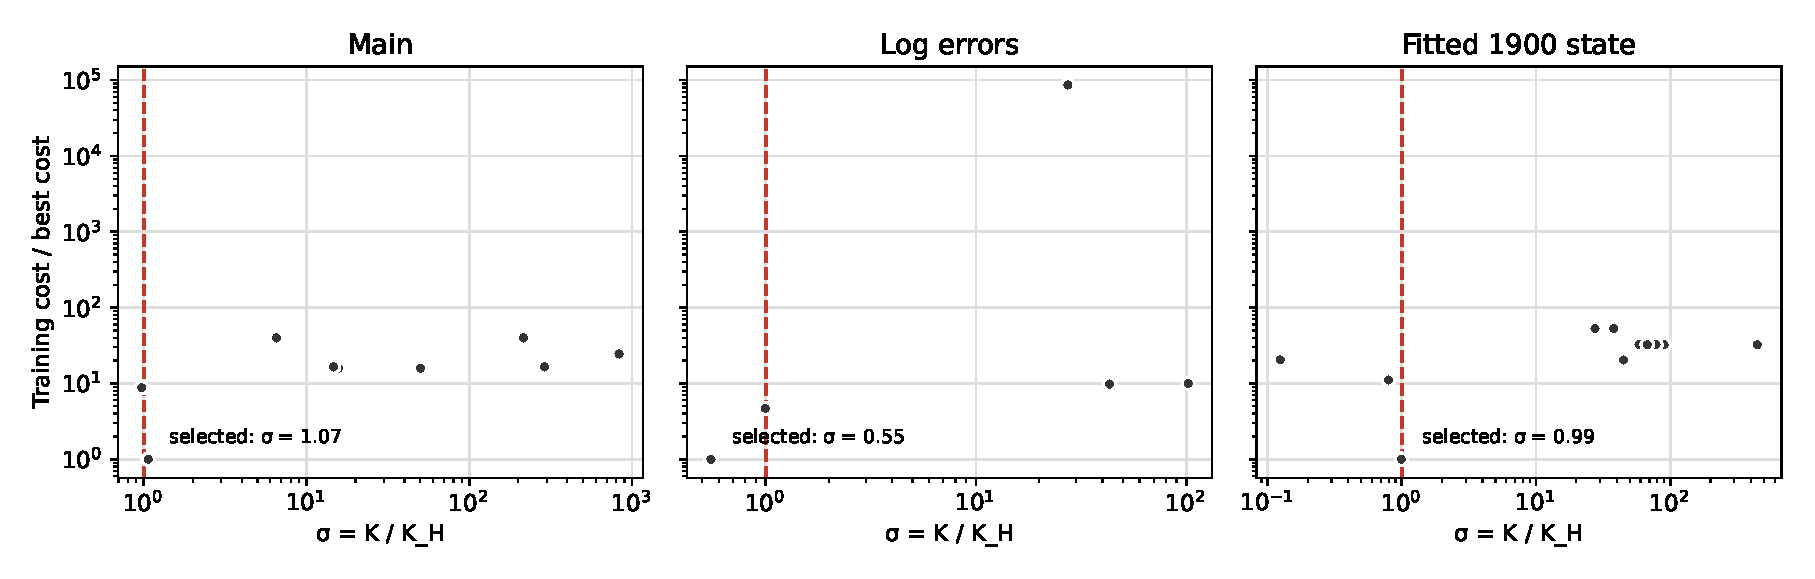
\includegraphics[width=\textwidth]{advay_baseline_sigma}
\caption{Training cost relative to the best, against $\sigma=K/K_H$, for every converged
start. The dashed line is the Hopf threshold $\sigma=1$. The best fits sit near $\sigma=1$,
on different sides depending on the variant.}\label{fig:advay-sigma}
\end{figure}

\subsection{Held-out evaluation, 1916--1920}\label{sec:advay-eval}

\paragraph{Protocol.} A scoring plan fixing the forecasts compared, the headline comparison,
the metrics and the interpretation rule was committed and published before the test file was
opened. All forecasts integrate frozen parameters from 1900 through 1920 with the shared
solver; nothing restarts from a test value, and no neural-network extrapolation is used.
For each species separately we report
$\mathrm{RMSE}=\big(\tfrac15\sum(\hat Y-Y)^2\big)^{1/2}$ and
$\mathrm{MAE}=\tfrac15\sum|\hat Y-Y|$ in thousands of pelts. With five test points a method
is called \emph{better} only if both its RMSE and MAE are smaller \emph{and} it is closer in
at least three of the five years; otherwise the methods are \emph{similar}. Two reference
forecasts use training data only: the 1915 value held constant (persistence) and the
1900--1915 mean. The headline comparison is the main least-squares fit against the
PINN-derived ODE forecast of the historical PINN study (seed chosen by training loss
before scoring). Every frozen forecast was checksum-verified, and the scores reproduce the
PINN study's own evaluation exactly.

\begin{table}[ht]
\centering
\begin{tabular}{llrrrr}
\hline
Variant & Method & Hare RMSE & Hare MAE & Lynx RMSE & Lynx MAE \\
\hline
Main (headline) & Least squares & 3.07 & 2.59 & 3.04 & 2.56 \\
 & PINN-derived ODE (seed17) & 2.85 & 2.59 & 4.32 & 4.05 \\
Log errors & Least squares & 6.87 & 6.63 & 1.60 & 1.38 \\
 & PINN-derived ODE (seed29) & 18.35 & 14.29 & 10.03 & 8.97 \\
Fitted 1900 state & Least squares & 2.25 & 2.08 & 3.24 & 2.71 \\
 & PINN-derived ODE (seed17) & 3.69 & 3.06 & 4.70 & 4.53 \\
\hline
Reference & Persistence (1915 value) & 7.38 & 6.72 & 37.16 & 36.32 \\
Reference & Training mean & 25.87 & 25.23 & 10.58 & 10.21 \\
\hline
\end{tabular}

\caption{Held-out errors, 1916--1920, thousands of pelts.}\label{tab:advay-metrics}
\end{table}

\paragraph{Results.} (Table~\ref{tab:advay-metrics}, Figures~\ref{fig:advay-overlay}
and~\ref{fig:advay-metrics}.)
\begin{itemize}
\item \textbf{Both methods forecast the crash and recovery.} In the main variant both predict
the 1916--1920 lynx collapse and the hare recovery to within about 3--4 thousand pelts, far
better than persistence (lynx RMSE 37.2) or the training mean (lynx 10.6, hare 25.9). The
fitted dynamics carry real information about the next half-cycle.
\item \textbf{Headline: mixed and close.} Hare: similar (RMSE 3.07 least squares,
2.85 PINN; MAE 2.59 both). Lynx: least squares better (3.04 against 4.32, closer in all five
years); the PINN-derived lynx forecast falls to 3--5 thousand after 1918 where 9.7--10.1 were
observed.
\item \textbf{Sensitivity variants.} Least squares is better or similar in both. The log-error
PINN fit places the 1913 peaks about a year early and its forecast errors are large (hare RMSE 18.4).
\item \textbf{Why they differ.} Evaluated on $C$, the selected PINN parameters fit the
training years 1.9--3.4 times worse than the least-squares optimum, as expected for an
estimator that minimises a combined data and physics loss, and they cycle more strongly
($\sigma\approx1.35$). A better training fit did not give a better hare forecast in the main
variant. With five points, none of these differences is strong evidence.
\end{itemize}

\begin{figure}[ht]
\centering
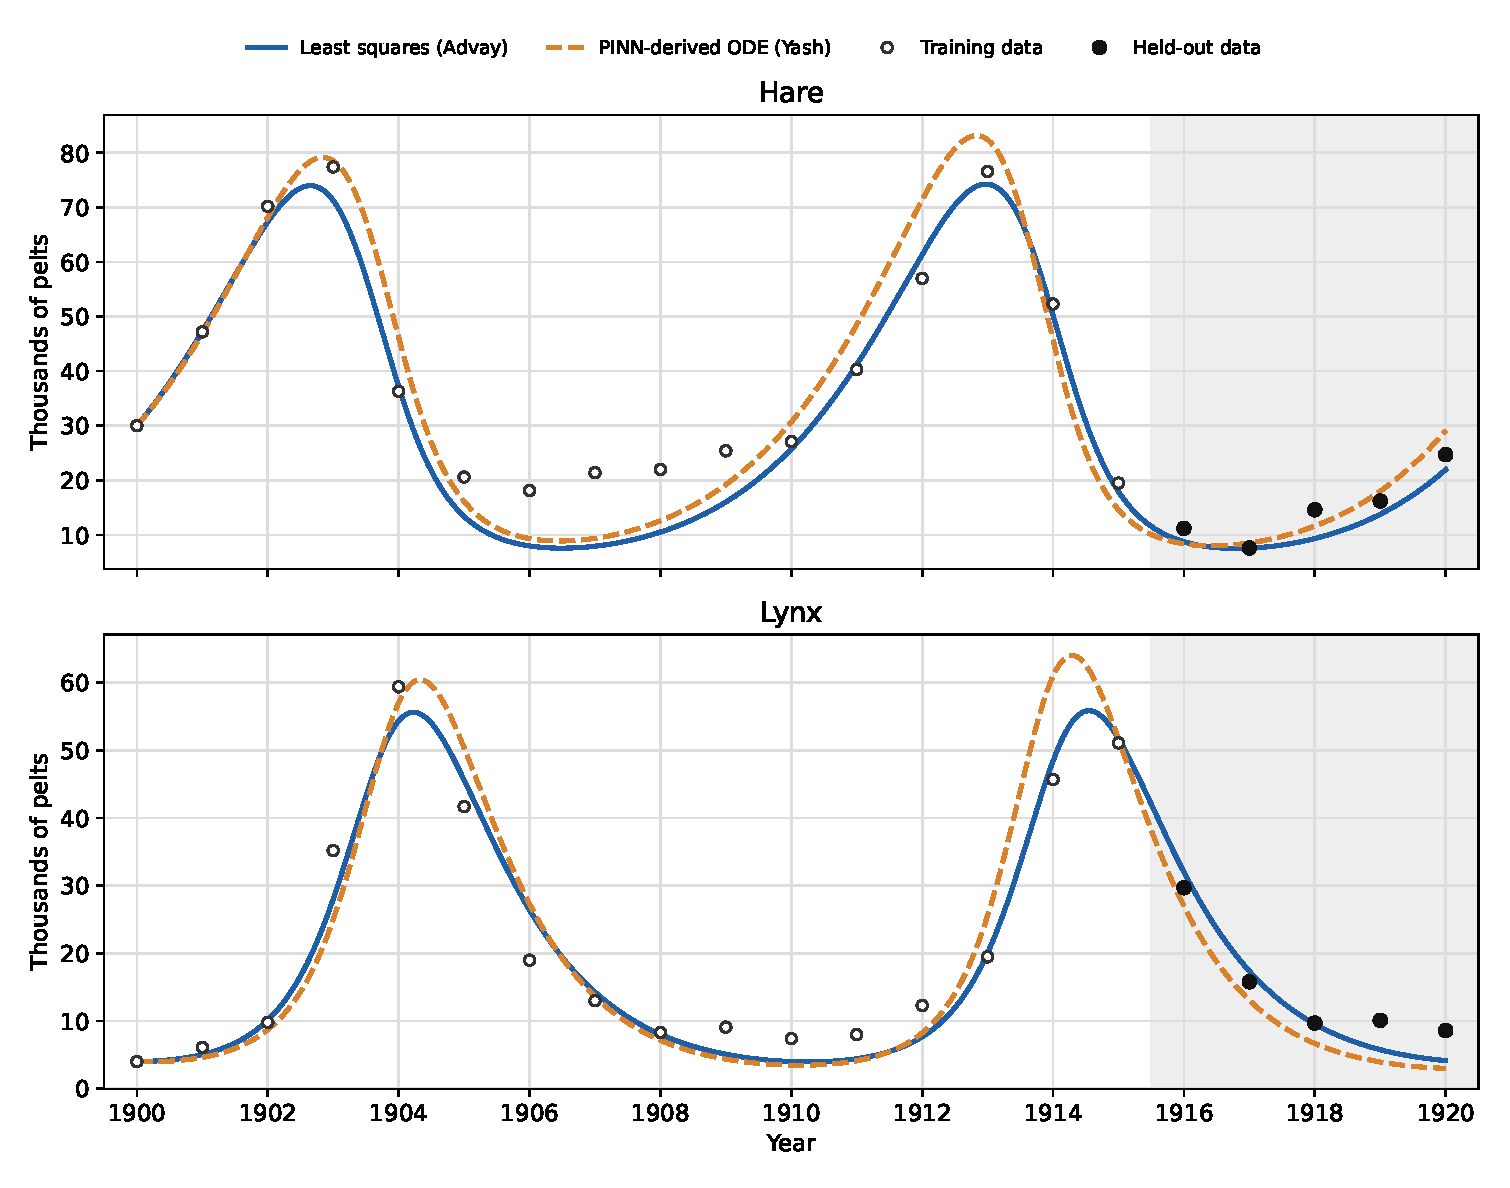
\includegraphics[width=0.9\textwidth]{advay_heldout_overlay}
\caption{Least-squares (solid) and PINN-derived (dashed) fits, main variant. Open circles:
training data; filled circles: held-out data (shaded). Both were fitted to 1900--1915 only
and integrated forward from 1900.}\label{fig:advay-overlay}
\end{figure}

\begin{figure}[ht]
\centering
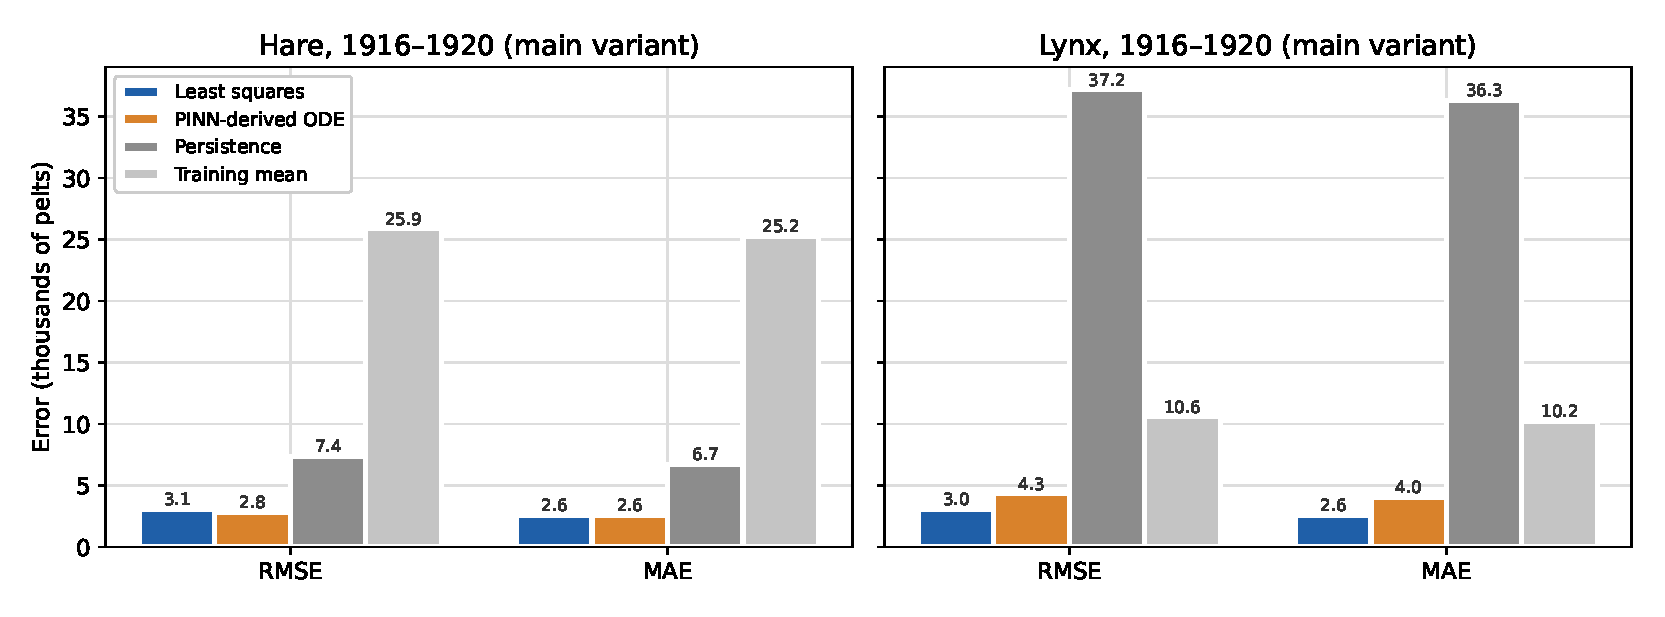
\includegraphics[width=\textwidth]{advay_heldout_metrics}
\caption{Held-out RMSE and MAE, main variant, with the persistence and training-mean
reference forecasts.}\label{fig:advay-metrics}
\end{figure}

\subsection{Limitations}\label{sec:advay-limits}

\begin{itemize}
\item \textbf{A very small test.} Five annual points, about half a cycle, beginning at the
1915 lynx peak. The comparison measures one crash and recovery, not long-run accuracy.
\item \textbf{Trade counts, not populations.} O1 assumes constant catchability; trapping
effort, prices and lynx behaviour almost certainly varied. Annual totals are treated as
point samples, a mismatch of up to a year in timing.
\item \textbf{Source uncertainty.} Two compilations of the same records disagree by more than
the forecast errors in some years; all results are conditional on the Stan series.
\item \textbf{Initial state.} The main analysis treats the noisy 1900 counts as exact. Fitting
them instead moves $\sigma$ from 1.07 to 0.99 and lowers the hare error.
\item \textbf{Identifiability.} $K$, $a$ and $b$ are individually poorly determined and $b$
(and $a$ in the main fit) lies on the box boundary, so their values depend on the chosen
bounds. A good curve fit is not evidence of uniquely recovered biological rates.
\item \textbf{Observation model.} Changing only the error model (additive to log) changes
$\sigma$ from 1.07 to 0.55 and the hare/lynx error balance, so the qualitative dynamics
inferred are sensitive to how the counts are assumed to be measured.
\item \textbf{Missing ecology.} A closed two-species, constant-parameter model omits
vegetation, other predators, weather, disease and spatial structure. Its success over
1916--1920 shows that it captures the dominant short-term feedback, not that it is complete.
\end{itemize}

\paragraph{Reproduction.} \texttt{scripts/advay\_data\_checks.py},
\texttt{advay\_make\_split.py}, \texttt{advay\_fit\_baseline.py --protocol v2},
\texttt{advay\_compare\_benchmark.py} and \texttt{advay\_score\_heldout.py} regenerate every
number and figure in this section; the declared protocols are in
\texttt{docs/advay\_baseline\_protocol.md} and \texttt{docs/advay\_scoring\_plan.md}.
   (standalone build: advay_main.tex)
% Figures: graphs/advay_*.{eps,pdf}; table: tables/advay_heldout_metrics.tex.
\section{Data, Least-Squares Baseline and Validation}\label{sec:advay}

This section states what the historical observations are, how they were prepared, how the
model was fitted to them by nonlinear least squares, and how well the fitted model forecasts
years it never saw. Every analysis choice that could be influenced by the held-out years was
written down and committed to the project repository before those years were opened.

\subsection{Data source and meaning}\label{sec:advay-data}

We use annual counts of snowshoe hare and Canadian lynx pelts traded by the Hudson's Bay
Company, 1900--1920, in thousands of pelts, as distributed with the Stan case study
\cite{carpenter2018}. Carpenter traces the numbers through Howard's lecture notes
\cite{howard2009} to a biology textbook; the original source is the Company's fur returns,
discussed by Hewitt \cite{hewitt1921}. The values are used unchanged
(\texttt{data/historical/pelts\_1900\_1920.csv}); the file's provenance, checksums and every
transformation (removing comment lines, reordering columns) are recorded alongside it.

These are \emph{trade counts}, not censuses. Trapping effort, fur prices, the number of
reporting posts and animal behaviour all affect them; Hewitt notes that hungry lynx are
easier to trap when hares are scarce. A second widely used compilation, the tsibbledata
\texttt{pelt} series \cite{tsibbledata_pelt}, differs noticeably over the same years
(Figure~\ref{fig:advay-sources}): the correlation between the two is 0.81 for lynx but only
0.32 for hare, and individual hare values differ by more than our forecast errors. We use
the Stan series because the project protocol names it, and treat the disagreement as a source
of uncertainty that no model in this report can remove.

\begin{figure}[ht]
\centering
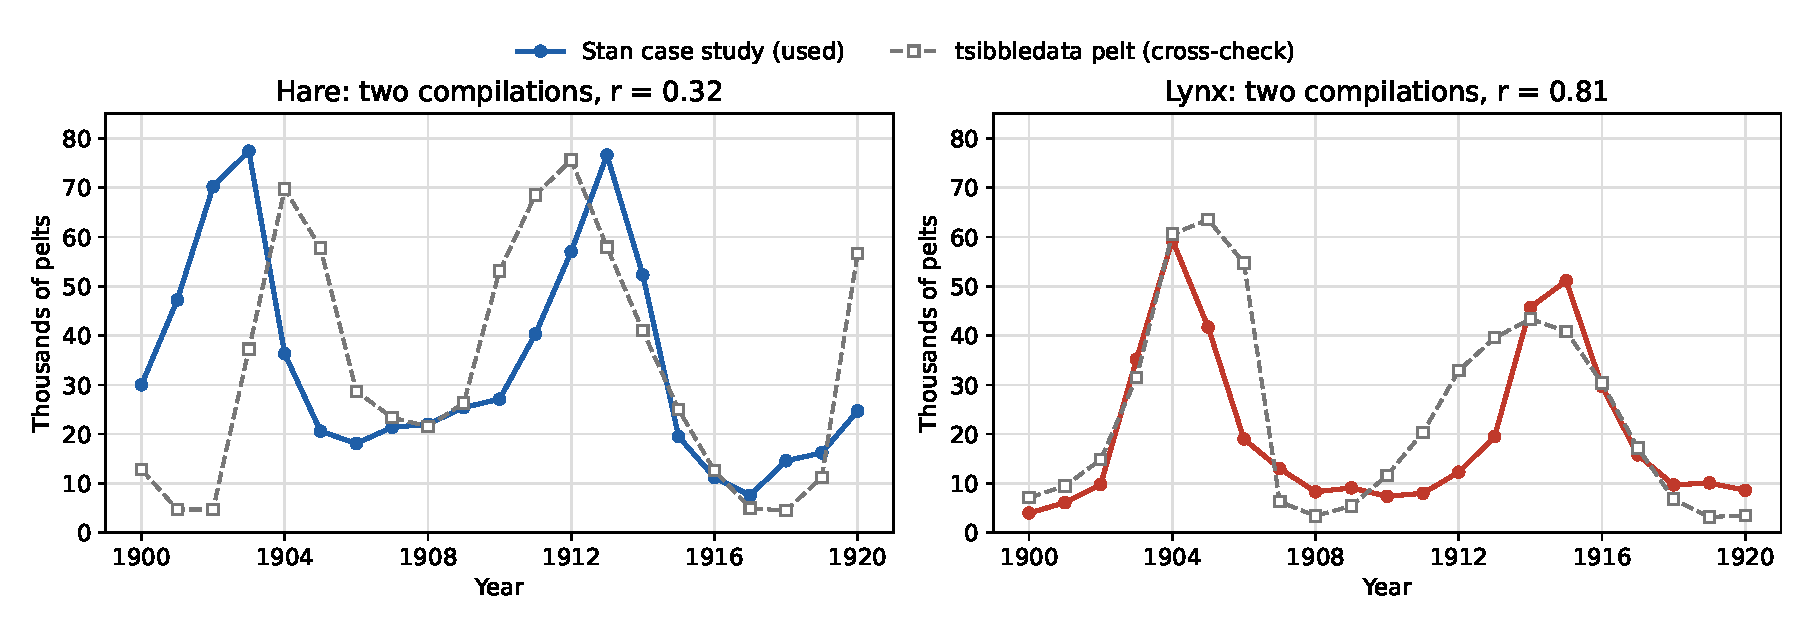
\includegraphics[width=\textwidth]{advay_source_comparison}
\caption{The Stan case-study series used here (solid) and the tsibbledata \texttt{pelt}
compilation (dashed) for 1900--1920. Both show two cycles, but yearly values differ,
especially for hare.}\label{fig:advay-sources}
\end{figure}

\paragraph{Observation model.} Following the agreed convention (assumption O1), pelt counts
are taken to be proportional to animal numbers with unknown constant factors, and the model
states are defined directly in pelt units:
\[
Y_{H,i}=H(t_i)+\varepsilon_{H,i},\qquad Y_{P,i}=P(t_i)+\varepsilon_{P,i},\qquad t_i=\mathrm{Year}_i-1900,
\]
with each annual total treated as a sample of the state at $t_i$. No observation scale factor
is fitted. Under O1, $r$, $m$ and the dimensionless groups of the model section are unchanged
by the unknown factors; $K$, $b$, $a$ and $e$ are \emph{effective} coefficients in pelt
units and are not interpreted as absolute biological quantities.

\subsection{Preparation and exploratory checks}\label{sec:advay-checks}

The 21 rows are consecutive, with no missing values, no zeros and no duplicates. The data
were split once into a training file (1900--1915, 16 rows) and a test file (1916--1920,
5 rows), with checksums recorded; all fitting code reads only the training file. Every
statistic below uses the training years only.

\begin{itemize}
\item \textbf{Cycles and lag.} Hare peaks in 1903 and 1913 (a ten-year spacing); lynx peaks
in 1904 and at the 1915 boundary. The correlation of $H(t)$ with $P(t+k)$ is largest at
$k=2$ years ($r=0.94$; $0.76$ at $k=1$). In the hare--lynx plane the data trace
counter-clockwise loops, as predator--prey models predict (Figure~\ref{fig:advay-raw}).
\item \textbf{Outliers.} None: robust $z$-scores of year-to-year log growth stay below 3
(largest 2.94, the 1903--1904 hare crash).
\item \textbf{Scale.} Training ranges are 18.1--77.4 (hare) and 4.0--59.4 (lynx). Hare counts
are about twice lynx counts, so residuals are divided by each species' training maximum
$(s_H,s_P)=(77.4,59.4)$ to weight the species equally. No log transform is used in the main
analysis; a log-residual fit is a declared sensitivity check.
\item \textbf{Split position.} Training ends exactly at the 1915 lynx peak, so the test years
are the following crash and the start of recovery: a turning point the fit never sees in
that cycle.
\end{itemize}

\begin{figure}[ht]
\centering
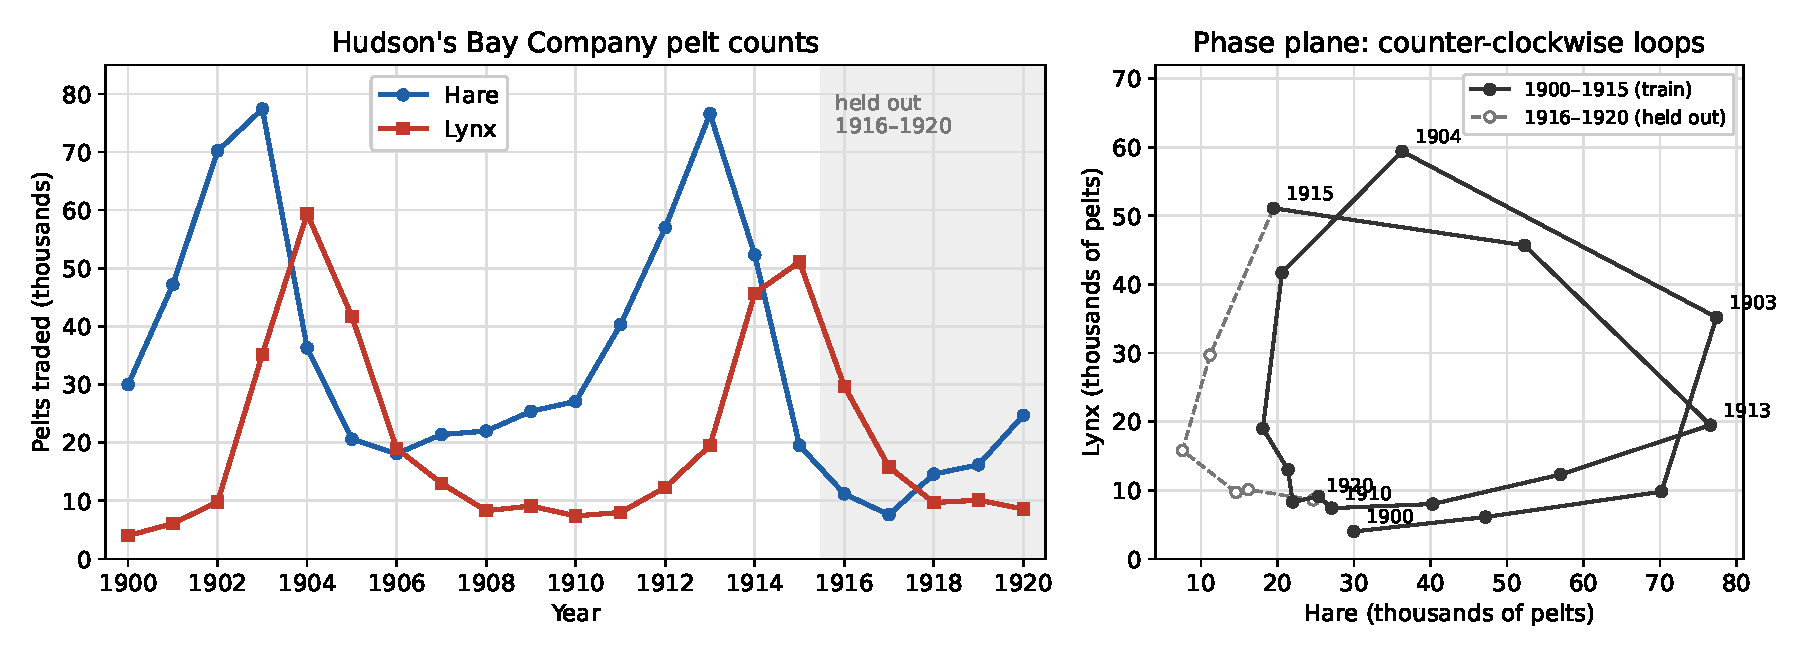
\includegraphics[width=\textwidth]{advay_raw_series}
\caption{Left: annual pelt counts, 1900--1920; the shaded band is held out. Right: the same
data in the hare--lynx plane (training solid, held-out dashed).}\label{fig:advay-raw}
\end{figure}

\subsection{Least-squares baseline}\label{sec:advay-ls}

\paragraph{Problem.} With $\theta=(r,K,a,b,e,m)$ and the shared RK45 solver (relative
tolerance $10^{-8}$, absolute $10^{-10}$, maximum step $0.1$ years), let $\hat H(t;\theta)$,
$\hat P(t;\theta)$ solve the model from the observed 1900 state $(30.0,4.0)$. The main
estimate minimises
\[
C(\theta)=\tfrac12\sum_{i=1900}^{1915}\Big[\big(\tfrac{\hat H(t_i;\theta)-Y_{H,i}}{s_H}\big)^2+
\big(\tfrac{\hat P(t_i;\theta)-Y_{P,i}}{s_P}\big)^2\Big]
\]
over the shared box bounds $r,m\in[0.05,3]$, $K\in[20,500]$, $a\in[0.05,10]$,
$b\in[0.5,300]$, $e\in[0.02,5]$. Two declared sensitivity variants change one assumption
each: \emph{log errors} replaces the scaled residuals by $\log\hat Y-\log Y$, and
\emph{fitted 1900 state} adds $(H_0,P_0)$ as unknowns within $[0.5,1.5]$ times the observed
values.

\paragraph{Method.} The bounded trust-region reflective algorithm (SciPy
\texttt{least\_squares}) is run in log-parameter space $x=\log\theta$, because the bounds
span up to a 600-fold range. Finite-difference steps of $10^{-4}$ in $x$ stay well above the
solver tolerance. The objective is multimodal, so each variant uses 80 starts: the shared
initial guess, 39 Latin-hypercube points uniform in $\log\theta$ and 39 uniform in $\theta$.
The fit with the lowest training cost is selected.

\paragraph{Protocol record.} The settings were committed before the first run. That run
(40 log-space starts) missed the best \emph{fitted 1900 state} fit, which an independent
benchmark had found at training cost $0.063$ against our $0.70$; evaluating our objective at
the benchmark's parameters gave $0.063$, so the code agreed and the start design was at
fault (the optimum sits near the upper bounds, which log-uniform starts rarely visit). The
uniform-scale starts were added as a declared amendment, judged on training cost alone and
before any test score of the baseline was computed. Both runs are kept.

\begin{table}[ht]
\centering
\begin{tabular}{lrrrrrrrl}
\toprule
Variant & $C$ & $r$ & $K$ & $a$ & $b$ & $e$ & $m$ & $\sigma=K/K_H$\\
\midrule
Main & 0.0845 & 0.647 & 382 & 10.0$^*$ & 300$^*$ & 0.967 & 0.857 & 1.07 (cycle)\\
Log errors & 0.903 & 0.520 & 197 & 7.17 & 300$^*$ & 1.80 & 1.15 & 0.55 (damped)\\
Fitted 1900 state & 0.0634 & 0.520 & 362 & 8.15 & 300$^*$ & 1.32 & 1.05 & 0.99 (damped)\\
\bottomrule
\end{tabular}
\caption{Least-squares estimates. $^*$ at the upper bound. Units: $r,m$ per year; $K,b$
thousands of hare pelts; $a,e$ effective pelt-unit coefficients. The fitted 1900 state in the
last variant is $(37.1,3.64)$.}\label{tab:advay-ls}
\end{table}

\paragraph{Results.} Table~\ref{tab:advay-ls} and Figure~\ref{fig:advay-fit} give the selected
fits. Three findings matter for interpretation.
\begin{enumerate}
\item \emph{The optimum is computationally well defined.} In every variant all starts within
1\% of the best cost (18, 42 and 16 of 80) found the same parameters to four significant
figures, and a separately written least-squares code by another team member reaches the same
optimum (training costs within $2\times10^{-7}$, forecasts within 0.002 thousand pelts).
\item \emph{The saturation of predation is not identified.} $b$ sits on its upper bound in
every variant. With $b$ about four times the largest hare count, $aH/(b+H)\approx(a/b)H$ over
the data: predation is nearly linear in hare abundance. In the linearised fit the
correlation between $\log a$ and $\log b$ is 0.998 and the approximate standard errors of
$\log K$, $\log a$, $\log b$ exceed 1 (a factor of three or more), whereas $r$, $e$, $m$ are
determined to about 10--40\%. Only the ratio $a/b\approx0.024$--$0.033$ is well determined.
Because the optimum lies on the boundary, its location depends on the chosen box.
\item \emph{Limit cycle or damped oscillation is not decided.} Using the Hopf threshold
$K_H=b(ea+m)/(ea-m)$ from the stability analysis, $\sigma$ is 1.07 for the main fit (just past the threshold),
0.99 with a fitted 1900 state (just below) and 0.55 with log errors. All three reproduce the
observed timing equally well (hare peaks fitted at 1902.5--1902.8 and 1912.6--1913.0, lynx
1.6 years later, period about ten years). Two cycles of data cannot distinguish a stable
limit cycle from a slowly damped oscillation (Figure~\ref{fig:advay-sigma}).
\end{enumerate}

\begin{figure}[ht]
\centering
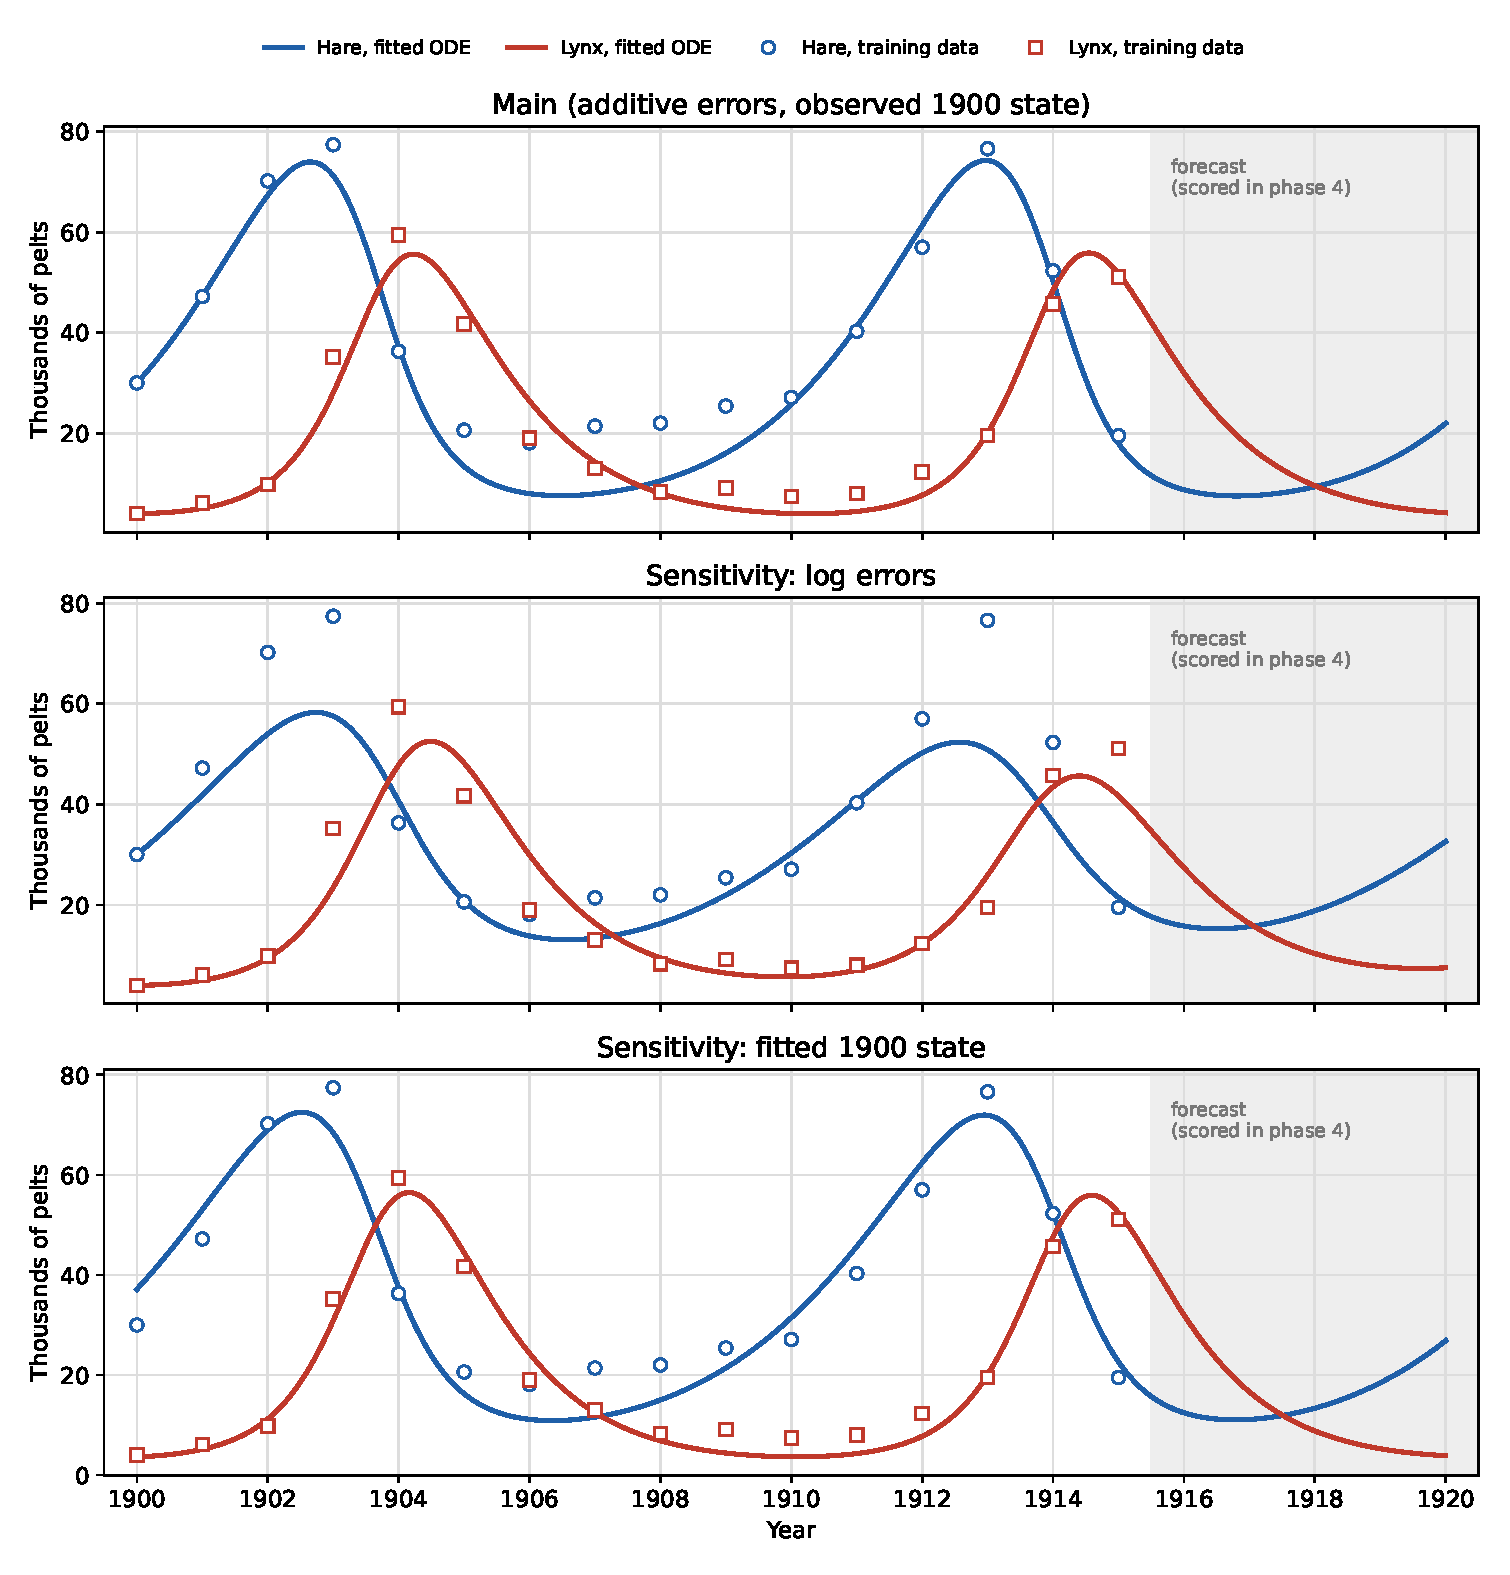
\includegraphics[width=0.9\textwidth]{advay_baseline_fit}
\caption{Least-squares fits to the 1900--1915 pelt counts (markers) and their continuation
through 1920 (shaded, held out) for the main analysis and both sensitivity variants.}
\label{fig:advay-fit}
\end{figure}

\begin{figure}[ht]
\centering
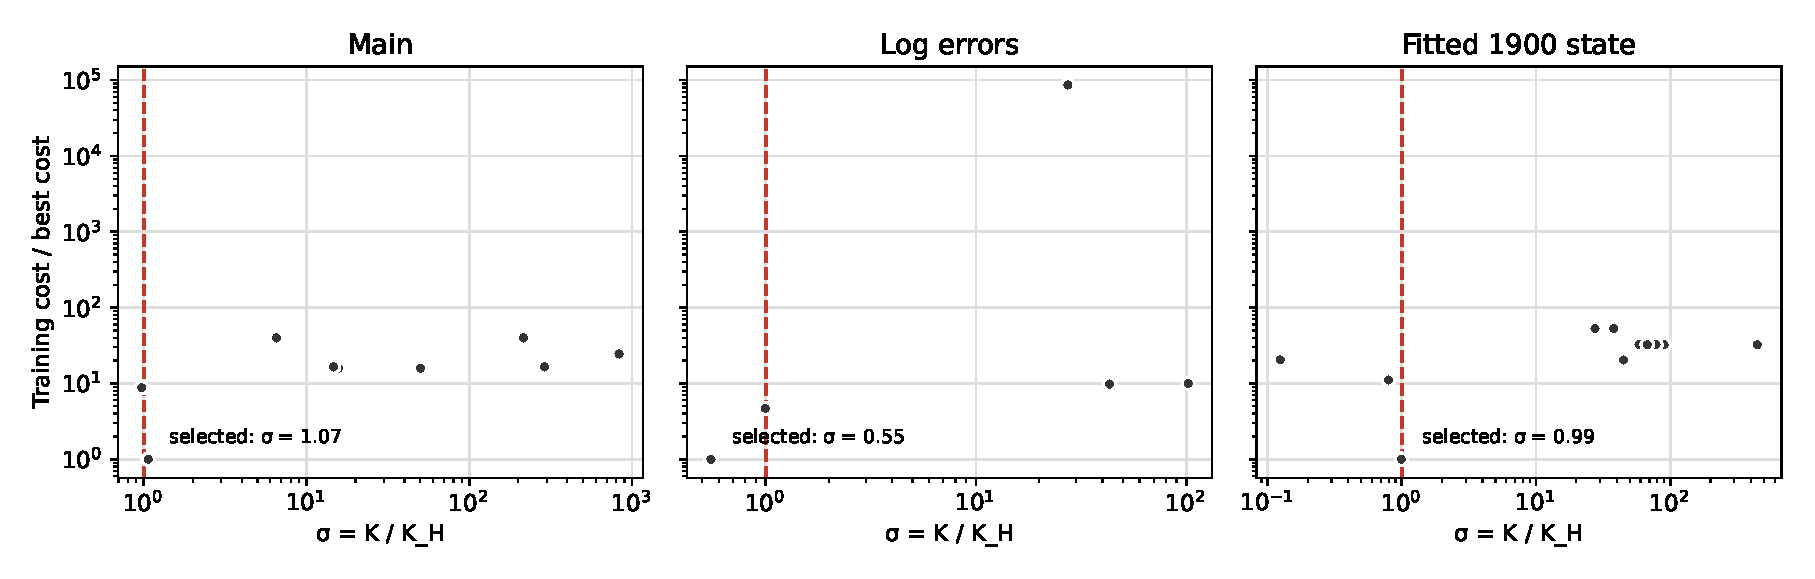
\includegraphics[width=\textwidth]{advay_baseline_sigma}
\caption{Training cost relative to the best, against $\sigma=K/K_H$, for every converged
start. The dashed line is the Hopf threshold $\sigma=1$. The best fits sit near $\sigma=1$,
on different sides depending on the variant.}\label{fig:advay-sigma}
\end{figure}

\subsection{Held-out evaluation, 1916--1920}\label{sec:advay-eval}

\paragraph{Protocol.} A scoring plan fixing the forecasts compared, the headline comparison,
the metrics and the interpretation rule was committed and published before the test file was
opened. All forecasts integrate frozen parameters from 1900 through 1920 with the shared
solver; nothing restarts from a test value, and no neural-network extrapolation is used.
For each species separately we report
$\mathrm{RMSE}=\big(\tfrac15\sum(\hat Y-Y)^2\big)^{1/2}$ and
$\mathrm{MAE}=\tfrac15\sum|\hat Y-Y|$ in thousands of pelts. With five test points a method
is called \emph{better} only if both its RMSE and MAE are smaller \emph{and} it is closer in
at least three of the five years; otherwise the methods are \emph{similar}. Two reference
forecasts use training data only: the 1915 value held constant (persistence) and the
1900--1915 mean. The headline comparison is the main least-squares fit against the
PINN-derived ODE forecast of the historical PINN study (seed chosen by training loss
before scoring). Every frozen forecast was checksum-verified, and the scores reproduce the
PINN study's own evaluation exactly.

\begin{table}[ht]
\centering
\begin{tabular}{llrrrr}
\hline
Variant & Method & Hare RMSE & Hare MAE & Lynx RMSE & Lynx MAE \\
\hline
Main (headline) & Least squares & 3.07 & 2.59 & 3.04 & 2.56 \\
 & PINN-derived ODE (seed17) & 2.85 & 2.59 & 4.32 & 4.05 \\
Log errors & Least squares & 6.87 & 6.63 & 1.60 & 1.38 \\
 & PINN-derived ODE (seed29) & 18.35 & 14.29 & 10.03 & 8.97 \\
Fitted 1900 state & Least squares & 2.25 & 2.08 & 3.24 & 2.71 \\
 & PINN-derived ODE (seed17) & 3.69 & 3.06 & 4.70 & 4.53 \\
\hline
Reference & Persistence (1915 value) & 7.38 & 6.72 & 37.16 & 36.32 \\
Reference & Training mean & 25.87 & 25.23 & 10.58 & 10.21 \\
\hline
\end{tabular}

\caption{Held-out errors, 1916--1920, thousands of pelts.}\label{tab:advay-metrics}
\end{table}

\paragraph{Results.} (Table~\ref{tab:advay-metrics}, Figures~\ref{fig:advay-overlay}
and~\ref{fig:advay-metrics}.)
\begin{itemize}
\item \textbf{Both methods forecast the crash and recovery.} In the main variant both predict
the 1916--1920 lynx collapse and the hare recovery to within about 3--4 thousand pelts, far
better than persistence (lynx RMSE 37.2) or the training mean (lynx 10.6, hare 25.9). The
fitted dynamics carry real information about the next half-cycle.
\item \textbf{Headline: mixed and close.} Hare: similar (RMSE 3.07 least squares,
2.85 PINN; MAE 2.59 both). Lynx: least squares better (3.04 against 4.32, closer in all five
years); the PINN-derived lynx forecast falls to 3--5 thousand after 1918 where 9.7--10.1 were
observed.
\item \textbf{Sensitivity variants.} Least squares is better or similar in both. The log-error
PINN fit places the 1913 peaks about a year early and its forecast errors are large (hare RMSE 18.4).
\item \textbf{Why they differ.} Evaluated on $C$, the selected PINN parameters fit the
training years 1.9--3.4 times worse than the least-squares optimum, as expected for an
estimator that minimises a combined data and physics loss, and they cycle more strongly
($\sigma\approx1.35$). A better training fit did not give a better hare forecast in the main
variant. With five points, none of these differences is strong evidence.
\end{itemize}

\begin{figure}[ht]
\centering
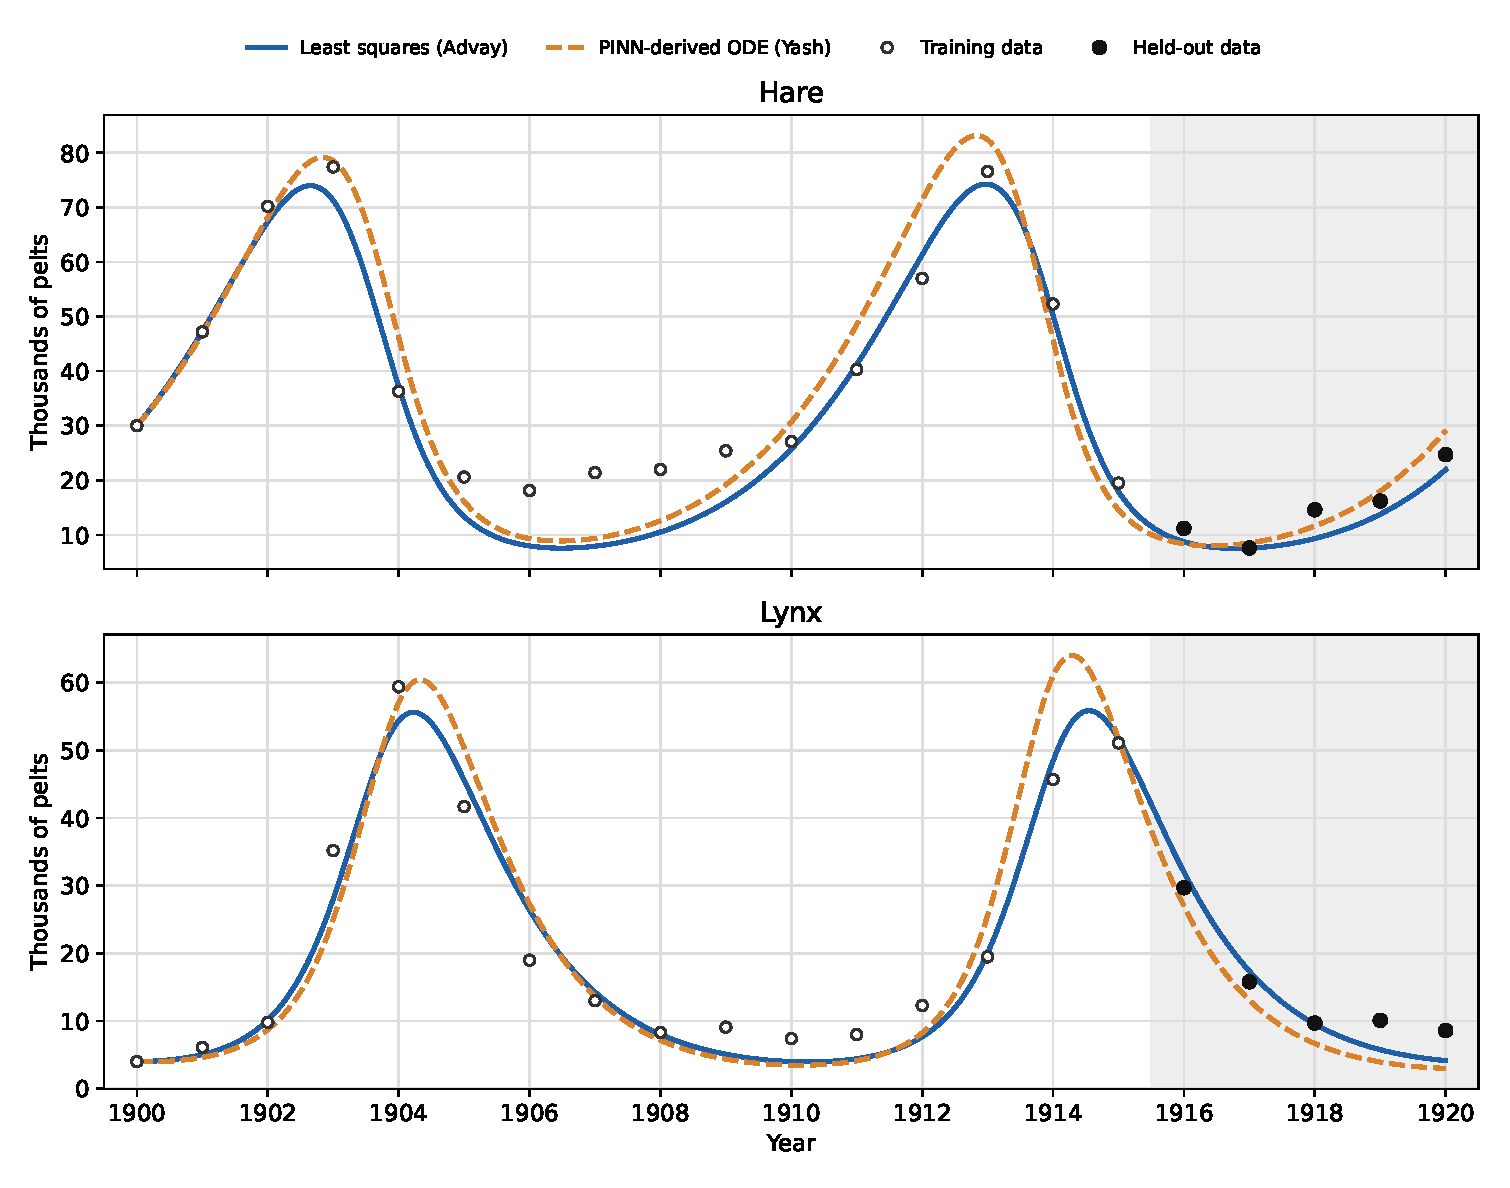
\includegraphics[width=0.9\textwidth]{advay_heldout_overlay}
\caption{Least-squares (solid) and PINN-derived (dashed) fits, main variant. Open circles:
training data; filled circles: held-out data (shaded). Both were fitted to 1900--1915 only
and integrated forward from 1900.}\label{fig:advay-overlay}
\end{figure}

\begin{figure}[ht]
\centering
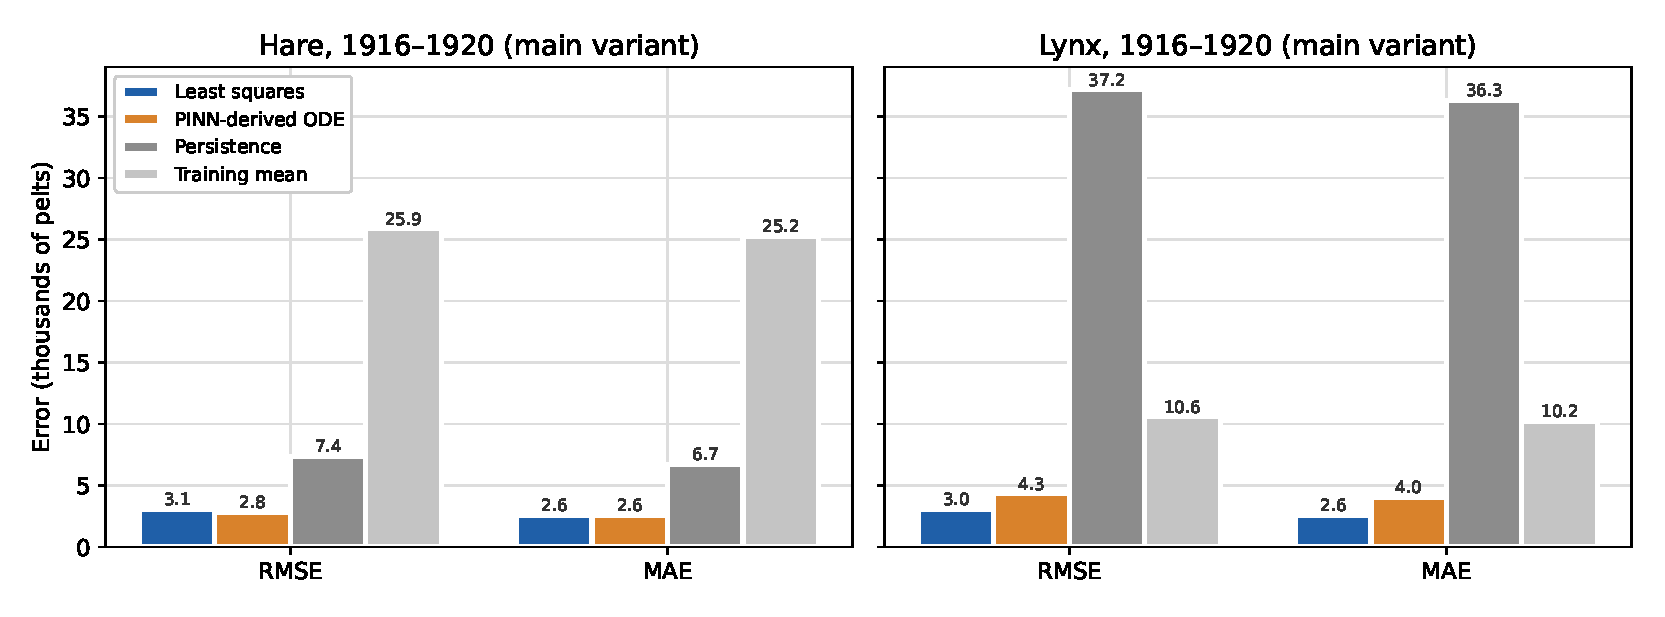
\includegraphics[width=\textwidth]{advay_heldout_metrics}
\caption{Held-out RMSE and MAE, main variant, with the persistence and training-mean
reference forecasts.}\label{fig:advay-metrics}
\end{figure}

\subsection{Limitations}\label{sec:advay-limits}

\begin{itemize}
\item \textbf{A very small test.} Five annual points, about half a cycle, beginning at the
1915 lynx peak. The comparison measures one crash and recovery, not long-run accuracy.
\item \textbf{Trade counts, not populations.} O1 assumes constant catchability; trapping
effort, prices and lynx behaviour almost certainly varied. Annual totals are treated as
point samples, a mismatch of up to a year in timing.
\item \textbf{Source uncertainty.} Two compilations of the same records disagree by more than
the forecast errors in some years; all results are conditional on the Stan series.
\item \textbf{Initial state.} The main analysis treats the noisy 1900 counts as exact. Fitting
them instead moves $\sigma$ from 1.07 to 0.99 and lowers the hare error.
\item \textbf{Identifiability.} $K$, $a$ and $b$ are individually poorly determined and $b$
(and $a$ in the main fit) lies on the box boundary, so their values depend on the chosen
bounds. A good curve fit is not evidence of uniquely recovered biological rates.
\item \textbf{Observation model.} Changing only the error model (additive to log) changes
$\sigma$ from 1.07 to 0.55 and the hare/lynx error balance, so the qualitative dynamics
inferred are sensitive to how the counts are assumed to be measured.
\item \textbf{Missing ecology.} A closed two-species, constant-parameter model omits
vegetation, other predators, weather, disease and spatial structure. Its success over
1916--1920 shows that it captures the dominant short-term feedback, not that it is complete.
\end{itemize}

\paragraph{Reproduction.} \texttt{scripts/advay\_data\_checks.py},
\texttt{advay\_make\_split.py}, \texttt{advay\_fit\_baseline.py --protocol v2},
\texttt{advay\_compare\_benchmark.py} and \texttt{advay\_score\_heldout.py} regenerate every
number and figure in this section; the declared protocols are in
\texttt{docs/advay\_baseline\_protocol.md} and \texttt{docs/advay\_scoring\_plan.md}.
